\documentclass[a4paper,12pt,twoside]{memoir}

% Castellano
\usepackage[spanish,es-tabla]{babel}
\selectlanguage{spanish}
\usepackage[utf8]{inputenc}
\usepackage[T1]{fontenc}
\usepackage{lmodern} % scalable font
\usepackage{microtype}
\usepackage{placeins}

\RequirePackage{booktabs}
\RequirePackage[table]{xcolor}
\RequirePackage{xtab}
\RequirePackage{multirow}

% Links
\PassOptionsToPackage{hyphens}{url}\usepackage[colorlinks]{hyperref}
\hypersetup{
	allcolors = {red}
}

% Ecuaciones
\usepackage{amsmath}

%Código
\usepackage{listings}

\usepackage{inconsolata}
\lstset{
	language=bash, %% Troque para PHP, C, Java, etc... bash é o padrão
	basicstyle=\ttfamily\small,
	numberstyle=\footnotesize,
	numbers=left,
	backgroundcolor=\color{gray!10},
	frame=single,
	tabsize=2,
	rulecolor=\color{black!30},
	title=\lstname,
	escapeinside={\%*}{*)},
	breaklines=true,
	breakatwhitespace=true,
	framextopmargin=2pt,
	framexbottommargin=2pt,
	inputencoding=utf8,
	extendedchars=true,
	literate={á}{{\'a}}1 {ã}{{\~a}}1 {é}{{\'e}}1 {ó}{{\'o}}1 {í}{{\'i}}1
}

%Árbol de directorios
\usepackage{dirtree}

% Rutas de fichero / paquete
\newcommand{\ruta}[1]{{\sffamily #1}}

% Párrafos
\nonzeroparskip

% Huérfanas y viudas
\widowpenalty100000
\clubpenalty100000

% Evitar solapes en el header
\nouppercaseheads

% Imagenes
\usepackage{graphicx}
\newcommand{\imagen}[2]{
	\begin{figure}[!h]
		\centering
		\includegraphics[width=0.9\textwidth]{#1}
		\caption{#2}\label{fig:#1}
	\end{figure}
	\FloatBarrier
}
\usepackage{graphicx}
\usepackage{subfig}
\usepackage{caption}
\usepackage{subcaption}
\usepackage{float}

\newcommand{\imagenflotante}[2]{
	\begin{figure}%[!h]
		\centering
		\includegraphics[width=0.9\textwidth]{#1}
		\caption{#2}\label{fig:#1}
	\end{figure}
}



% El comando \figura nos permite insertar figuras comodamente, y utilizando
% siempre el mismo formato. Los parametros son:
% 1 -> Porcentaje del ancho de página que ocupará la figura (de 0 a 1)
% 2 --> Fichero de la imagen
% 3 --> Texto a pie de imagen
% 4 --> Etiqueta (label) para referencias
% 5 --> Opciones que queramos pasarle al \includegraphics
% 6 --> Opciones de posicionamiento a pasarle a \begin{figure}
\newcommand{\figuraConPosicion}[6]{%
  \setlength{\anchoFloat}{#1\textwidth}%
  \addtolength{\anchoFloat}{-4\fboxsep}%
  \setlength{\anchoFigura}{\anchoFloat}%
  \begin{figure}[#6]
    \begin{center}%
      \Ovalbox{%
        \begin{minipage}{\anchoFloat}%
          \begin{center}%
            \includegraphics[width=\anchoFigura,#5]{#2}%
            \caption{#3}%
            \label{#4}%
          \end{center}%
        \end{minipage}
      }%
    \end{center}%
  \end{figure}%
}

%
% Comando para incluir imágenes en formato apaisado (sin marco).
\newcommand{\figuraApaisadaSinMarco}[5]{%
  \begin{figure}%
    \begin{center}%
    \includegraphics[angle=90,height=#1\textheight,#5]{#2}%
    \caption{#3}%
    \label{#4}%
    \end{center}%
  \end{figure}%
}
% Para las tablas
\newcommand{\otoprule}{\midrule [\heavyrulewidth]}
%
% Nuevo comando para tablas pequeñas (menos de una página).
\newcommand{\tablaSmall}[5]{%
 \begin{table}
  \begin{center}
   \rowcolors {2}{gray!35}{}
   \begin{tabular}{#2}
    \toprule
    #4
    \otoprule
    #5
    \bottomrule
   \end{tabular}
   \caption{#1}
   \label{tabla:#3}
  \end{center}
 \end{table}
}

%
%Para el float H de tablaSmallSinColores
\usepackage{float}

%
% Nuevo comando para tablas pequeñas (menos de una página).
\newcommand{\tablaSmallSinColores}[5]{%
 \begin{table}[H]
  \begin{center}
   \begin{tabular}{#2}
    \toprule
    #4
    \otoprule
    #5
    \bottomrule
   \end{tabular}
   \caption{#1}
   \label{tabla:#3}
  \end{center}
 \end{table}
}

\newcommand{\tablaApaisadaSmall}[5]{%
\begin{landscape}
  \begin{table}
   \begin{center}
    \rowcolors {2}{gray!35}{}
    \begin{tabular}{#2}
     \toprule
     #4
     \otoprule
     #5
     \bottomrule
    \end{tabular}
    \caption{#1}
    \label{tabla:#3}
   \end{center}
  \end{table}
\end{landscape}
}

%
% Nuevo comando para tablas grandes con cabecera y filas alternas coloreadas en gris.
\newcommand{\tabla}[6]{%
  \begin{center}
    \tablefirsthead{
      \toprule
      #5
      \otoprule
    }
    \tablehead{
      \multicolumn{#3}{l}{\small\sl continúa desde la página anterior}\\
      \toprule
      #5
      \otoprule
    }
    \tabletail{
      \hline
      \multicolumn{#3}{r}{\small\sl continúa en la página siguiente}\\
    }
    \tablelasttail{
      \hline
    }
    \bottomcaption{#1}
    \rowcolors {2}{gray!35}{}
    \begin{xtabular}{#2}
      #6
      \bottomrule
    \end{xtabular}
    \label{tabla:#4}
  \end{center}
}

%
% Nuevo comando para tablas grandes con cabecera.
\newcommand{\tablaSinColores}[6]{%
  \begin{center}
    \tablefirsthead{
      \toprule
      #5
      \otoprule
    }
    \tablehead{
      \multicolumn{#3}{l}{\small\sl continúa desde la página anterior}\\
      \toprule
      #5
      \otoprule
    }
    \tabletail{
      \hline
      \multicolumn{#3}{r}{\small\sl continúa en la página siguiente}\\
    }
    \tablelasttail{
      \hline
    }
    \bottomcaption{#1}
    \begin{xtabular}{#2}
      #6
      \bottomrule
    \end{xtabular}
    \label{tabla:#4}
  \end{center}
}

%
% Nuevo comando para tablas grandes sin cabecera.
\newcommand{\tablaSinCabecera}[5]{%
  \begin{center}
    \tablefirsthead{
      \toprule
    }
    \tablehead{
      \multicolumn{#3}{l}{\small\sl continúa desde la página anterior}\\
      \hline
    }
    \tabletail{
      \hline
      \multicolumn{#3}{r}{\small\sl continúa en la página siguiente}\\
    }
    \tablelasttail{
      \hline
    }
    \bottomcaption{#1}
  \begin{xtabular}{#2}
    #5
   \bottomrule
  \end{xtabular}
  \label{tabla:#4}
  \end{center}
}



\definecolor{cgoLight}{HTML}{EEEEEE}
\definecolor{cgoExtralight}{HTML}{FFFFFF}

%
% Nuevo comando para tablas grandes sin cabecera.
\newcommand{\tablaSinCabeceraConBandas}[5]{%
  \begin{center}
    \tablefirsthead{
      \toprule
    }
    \tablehead{
      \multicolumn{#3}{l}{\small\sl continúa desde la página anterior}\\
      \hline
    }
    \tabletail{
      \hline
      \multicolumn{#3}{r}{\small\sl continúa en la página siguiente}\\
    }
    \tablelasttail{
      \hline
    }
    \bottomcaption{#1}
    \rowcolors[]{1}{cgoExtralight}{cgoLight}

  \begin{xtabular}{#2}
    #5
   \bottomrule
  \end{xtabular}
  \label{tabla:#4}
  \end{center}
}




\graphicspath{ {./img/} }

% Capítulos
\chapterstyle{bianchi}
\newcommand{\capitulo}[2]{
	\setcounter{chapter}{#1}
	\setcounter{section}{0}
	\setcounter{figure}{0}
	\setcounter{table}{0}
	\chapter*{#2}
	\addcontentsline{toc}{chapter}{#2}
	\markboth{#2}{#2}
}

% Apéndices
\renewcommand{\appendixname}{Apéndice}
\renewcommand*\cftappendixname{\appendixname}

\newcommand{\apendice}[1]{
	%\renewcommand{\thechapter}{A}
	\chapter{#1}
}

\renewcommand*\cftappendixname{\appendixname\ }

% Formato de portada
\makeatletter
\usepackage{xcolor}
\newcommand{\tutor}[1]{\def\@tutor{#1}}
\newcommand{\course}[1]{\def\@course{#1}}
\definecolor{cpardoBox}{HTML}{E6E6FF}
\def\maketitle{
  \null
  \thispagestyle{empty}
  % Cabecera ----------------
\noindent
\includegraphics[width=\textwidth]{cabecera}\vspace{1cm}%
  \vfill
  % Título proyecto y escudo informática ----------------
  \colorbox{cpardoBox}{%
    \begin{minipage}{.8\textwidth}
      \vspace{.5cm}\Large
      \begin{center}
      \textbf{TFG del Grado en Ingeniería Informática}\vspace{.6cm}\\
      \textbf{\LARGE\@title{}}
      \end{center}
      \vspace{.2cm}
    \end{minipage}

  }%
  \hfill\begin{minipage}{.20\textwidth}
    
\includegraphics[width=\textwidth]{escudoInfor}
  \end{minipage}
  \vfill
  % Datos de alumno, curso y tutores ------------------
  \begin{center}%
  {%
    \noindent\LARGE
    Presentado por \@author{}\\ 
    en Universidad de Burgos --- \@date{}\\
    Tutor: \@tutor{}\\
  }%
  \end{center}%
  \null
  \cleardoublepage
  }
\makeatother


% Datos de portada
\title{Detección y evaluación de ejercicios de rehabilitación para pacientes con la enfermedad de Parkinson \\ \\Documentación Técnica}
\author{Lucía Núñez Calvo}
\tutor{José Francisco Díez Pastor, José Luis Garrido Labrador y José Miguel Ramírez Sanz}
\date{\today}

\begin{document}

\maketitle



\cleardoublepage



%%%%%%%%%%%%%%%%%%%%%%%%%%%%%%%%%%%%%%%%%%%%%%%%%%%%%%%%%%%%%%%%%%%%%%%%%%%%%%%%%%%%%%%%



\frontmatter


\clearpage

% Indices
\tableofcontents

\clearpage

\listoffigures

\clearpage

\listoftables

\clearpage

\mainmatter

\appendix

\apendice{Plan de Proyecto Software}

\section{Introducción}

La planificación de un proyecto es una fase fundamental para su correcto desarrollo. En este apartado se comentará, por una parte, la planificación temporal del proyecto mediante los distintos \textit{sprints} que se han llevado a cabo, y por otra parte, se realizará un breve estudio sobre la viabilidad del proyecto.

En este proyecto se ha utilizado la metodología ágil \textit{Scrum}, esta metodología tiene como objetivo base la creación de diferentes iteraciones o \textbf{sprints} \cite{trigas2012metodologia}. Para una correcta planificación, se optó por realizar \textit{sprints} de dos o tres semanas de duración. Aunque las reuniones se realizaban semanalmente, los objetivos se planteaban con un margen de varias semanas y en las reuniones posteriores se iban comentando las dudas y los avances. 


\begin{enumerate}
    \item \textbf{Planificación Temporal}, se expondrán las diferentes tareas realizadas en cada uno de los \textit{sprint}, acompañadas del coste estimado que se propuso para ellas y el coste final que implicó su realización. 
    \item \textbf{Estudio de viabilidad}, en este apartado se comprobará si el proyecto realizado tiene una viabilidad legal y económica.
\end{enumerate}
\newpage
\section{Planificación temporal}
La planificación temporal se ha dividido en distintos \textit{sprints} de dos o tres semanas de duración cada uno, en los cuales se realizaron distintas tareas y reuniones. Las reuniones se realizaban semanalmente informando de las tareas realizadas y los problemas surgidos, a lo que aportaban distintas soluciones y tareas nuevas. 


\subsection{Sprint 0:  Noviembre - Enero}

El \textit{sprint 0} consistió en una primera toma de contacto con el proyecto que abarcó desde Noviembre del año 2021 a Enero del año 2022. En estos meses se realizaron reuniones periódicas cada dos semanas con el objetivo de comprender el proyecto de los alumnos José Luís Garrido Labrador y José Miguel Ramírez Sanz, pero sobretodo, asimilar y leer numerosos artículos sobre la metodología \textbf{DTW}(\textit{Dynamic Time Warping}) y como puede implantarse a la búsqueda de secuencias y comparación o extracción de características de la pose humana.


\subsection{Sprint 1: 03/02/2022 - 24/02/2022}

El \textit{sprint 1} consistió en una investigación sobre diferentes librerías en \textit{Python} que implementasen el algoritmo \textit{DTW}. Además se descargó la plantilla aportada por la Universidad de Burgos para poder desarrollar la memoria en \LaTeX.

\begin{table}[H]
\centering
\begin{tabular}{lcc}
\hline
\rowcolor[HTML]{EFEFEF} 
\multicolumn{1}{c}{\cellcolor[HTML]{EFEFEF}\textbf{Tareas}} & \textbf{Est.} & \textbf{Final} \\ \hline
\rowcolor[HTML]{ECF4FF} 
Investigación sobre paquetes DTW                            & 10            & 13             \\
\rowcolor[HTML]{EFEFEF} 
Investigar sobre la librería tslearn                        & 5             & 14             \\
\rowcolor[HTML]{ECF4FF} 
Investigar sobre la librería dtaidistance                   & 5             & 3              \\
\rowcolor[HTML]{EFEFEF} 
Investigar sobre la librería pydtw                          & 5             & 2              \\
\rowcolor[HTML]{ECF4FF} 
Investigar sobre la librería simpledtw                      & 5             & 2              \\
\rowcolor[HTML]{EFEFEF} 
Investigar sobre la librería scipy                          & 5             & 4              \\
\rowcolor[HTML]{ECF4FF} 
Descargar plantilla \LaTeX                                   & 1             & 1              \\ \hline
\end{tabular}
\caption{Tareas del \textit{sprint 1}.}
\label{sprint1}
\end{table}

La mayor dificultad en este \textit{sprint} fue la comprensión de las diferentes librerías, con qué tipo de datos se podían utilizar y cómo analizar y comprender los resultados obtenidos.  

\subsection{Sprint 2: 25/02/2022 - 10/03/2022}

El \textit{sprint 2} consistió en la realización de pruebas sobre los paquetes investigados y en la instalación de los programas necesarios para la ejecución del proyecto fin de máster, \texttt{TFM-2020}\footnote{Trabajo final de máster realizado por los alumnos José Luís Garrido Labrador y José Miguel Ramírez Sanz}. 

\begin{table}[H]
\centering
\resizebox{\textwidth}{!}{
\begin{tabular}{p{10cm}cc}
\hline
\rowcolor[HTML]{EFEFEF} 
\multicolumn{1}{c}{\cellcolor[HTML]{EFEFEF}\textbf{Tareas}}             & \multicolumn{1}{l}{\cellcolor[HTML]{EFEFEF}\textbf{Est.}} & \multicolumn{1}{l}{\cellcolor[HTML]{EFEFEF}\textbf{Final}} \\ \hline
\rowcolor[HTML]{ECF4FF} 
Ejecutar múltiples pruebas sobre las librerías analizadas               & 5                                                         & 7                                                          \\
\rowcolor[HTML]{EFEFEF} 
Investigar como representar resultados visualmente                      & 2                                                         & 2                                                          \\
\rowcolor[HTML]{ECF4FF} 
Crear un cuaderno con las pruebas realizadas                            & 1                                                         & 2                                                          \\
\rowcolor[HTML]{EFEFEF} 
Comenzar con el equipo \texttt{gamma}\footnote{\textit{gamma} es una máquina del grupo \textit{ADMIRABLE} de la Universidad de Burgos que ha sido utilizada para la realización de gran parte del proyecto.}                                           & 2                                                         & 4                                                          \\
\rowcolor[HTML]{ECF4FF} 
Instalar \textit{Nvidia, Cuda y Tensorflow }                                     & 2                                                         & 4                                                          \\
\rowcolor[HTML]{EFEFEF} 
Adaptar las versiones de los programas a las requeridas por el proyecto & 2                                                         & 7                                                          \\ \hline
\end{tabular}
}
\caption{Tareas del \textit{sprint 2}.}
\label{sprint2}
\end{table}

La mayor dificultad de este \textit{sprint} fue localizar las versiones compatibles entre los programas a instalar y conseguir instalarlo todo con éxito. 

\subsection{Sprint 3: 11/03/2022 - 24/03/2022}

El \textit{sprint 3} consistió en la descarga y ejecución del proyecto \textit{TFM-2020}. Además en este \textit{sprint} se crearon una serie de vídeos cortos que más tarde serían utilizados en las pruebas del proyecto.

\begin{table}[H]
\centering
\resizebox{\textwidth}{!}{
\begin{tabular}{p{10cm}cc}
\hline
\rowcolor[HTML]{EFEFEF} 
\multicolumn{1}{c}{\cellcolor[HTML]{EFEFEF}\textbf{Tareas}}        & \multicolumn{1}{l}{\cellcolor[HTML]{EFEFEF}\textbf{Est.}} & \multicolumn{1}{l}{\cellcolor[HTML]{EFEFEF}\textbf{Final}} \\ \hline
\rowcolor[HTML]{ECF4FF} 
Descargar y probar el proyecto de partida                          & 2                                                         & 12                                                         \\
\rowcolor[HTML]{EFEFEF} 
Crear vídeos cortos para poder probar el proyecto                  & 1                                                         & 1                                                          \\
\rowcolor[HTML]{ECF4FF} 
Solucionar error de \textit{Kafka}                                          & 2                                                         & 2                                                          \\
\rowcolor[HTML]{EFEFEF} 
Solucionar errores de compatibilidad                               & 2                                                         & 4                                                          \\
\rowcolor[HTML]{ECF4FF} 
Solucionar errores de memoria                                      & 2                                                         & 5                                                          \\
\rowcolor[HTML]{EFEFEF} 
Documenta errores surgidos en las instalaciones                    & 2                                                         & 2                                                          \\
\rowcolor[HTML]{ECF4FF} 
Documentar errores surgidos en las ejecuciones                     & 2                                                         & 3                                                          \\
\rowcolor[HTML]{EFEFEF} 
Probar los paquetes \textit{DTW} con datos de mayor tamaño unidimensionales & 5                                                         & 7                                                          \\ \hline
\end{tabular}
}
\caption{Tareas del \textit{sprint 3}.}
\label{sprint3}
\end{table}

La mayor dificultad de este \textit{sprint} fue conseguir solucionar los errores de versiones que surgían al intentar ejecutar el proyecto. Finalmente se consiguió subsanar muchos errores y ejecutar el proyecto, aunque este de momento no estaba listo para ser usado ya que se consiguió ejecutar pero no se consiguieron los resultados esperados en cuanto a la extracción de \textit{frames}.

\subsection{Sprint 4: 25/03/2022 - 07/04/2022}

El \textit{sprint 4} consistió en realizar numerosas pruebas sobre los algoritmos \textit{DTW} encontrados pero, en este caso sobre conjuntos de datos de mayor tamaño. También se analizaron tanto los resultados arrojados como los tiempos de ejecución trascurridos. 
Por otra parte fue clave el análisis que se hizo sobre el funcionamiento interno de los contenedores para comprender los posibles errores. 

\begin{table}[H]
\centering
\resizebox{\textwidth}{!}{
\begin{tabular}{p{10cm}cc}
\hline
\rowcolor[HTML]{EFEFEF} 
\multicolumn{1}{c}{\cellcolor[HTML]{EFEFEF}\textbf{Tareas}}        & \textbf{Est.} & \textbf{Final} \\ \hline
\rowcolor[HTML]{ECF4FF} 
Ejecutar pruebas con datos de mayor tamaño                         & 6             & 8              \\
\rowcolor[HTML]{EFEFEF} 
Ejecutar pruebas con datos multidimensionales                      & 7             & 10             \\
\rowcolor[HTML]{ECF4FF} 
Transferir archivos entre equipos usando el comando scp            & 1             & 1              \\
\rowcolor[HTML]{EFEFEF} 
Solucionar errores del proyecto                                    & 4             & 10             \\
\rowcolor[HTML]{ECF4FF} 
Analizar los contenedores Docker que se lanzaban en cada ejecución & 3             & 5              \\
\rowcolor[HTML]{EFEFEF} 
Analizar las imágenes Docker                                       & 4             & 4              \\
\rowcolor[HTML]{ECF4FF} 
Ejecutar contenedores Docker por separado                          & 3             & 3              \\
\rowcolor[HTML]{EFEFEF} 
Analizar los log de error                                          & 2             & 2              \\
\rowcolor[HTML]{ECF4FF} 
Redactar nuevos errores y sus soluciones                           & 1             & 1              \\ \hline

\end{tabular}
}
\caption{Tareas del \textit{sprint 4}.}
\label{sprint4}
\end{table}

La mayor dificultad de este \textit{sprint} fue familiarizarse con la tecnología \textit{Docker}. Se tuvieron que revisar cada una de las imágenes y analizar los contenedores individualmente. Finalmente se logró comprender la razón de muchos errores y el funcionamiento interno del proyecto. 

\subsection{Sprint 5: 08/04/2022 - 28/04/2022}
El \textit{sprint 5} consistió en la creación de nuevos conjuntos de datos, en concreto la creación de diversas series temporales para ejecutar múltiples pruebas sobre los algoritmos \textit{DTW} en conjuntos de datos mucho más dispersos y de mayor tamaño.

Tras comprobar los resultados arrojados se procedió a implementar la búsqueda de secuencias con datos reales. Para ello se extrajo el inicio, el final y la secuencia intermedia de cada secuencia obtenida, con estas secuencias de mucho menor tamaño se empezaron a realizar las pruebas de localización de secuencias y posteriormente analizar los resultados arrojados. 

\begin{table}[H]
\centering
\resizebox{\textwidth}{!}{
\begin{tabular}{p{10cm}cc}
\hline
\rowcolor[HTML]{EFEFEF} 
\multicolumn{1}{c}{\cellcolor[HTML]{EFEFEF}\textbf{Tareas}}                                 & \multicolumn{1}{l}{\cellcolor[HTML]{EFEFEF}\textbf{Est.}} & \multicolumn{1}{l}{\cellcolor[HTML]{EFEFEF}\textbf{Final}} \\ \hline
\rowcolor[HTML]{ECF4FF} 
Crear nuevos conjuntos de datos aleatorios, de mayor tamaño y con mayor ruido               & 1                                                         & 1                                                          \\
\rowcolor[HTML]{EFEFEF} 
Ejecutar múltiples pruebas sobre los nuevos conjuntos de datos                              & 3                                                         & 5                                                          \\
\rowcolor[HTML]{ECF4FF} 
Crear nuevos conjuntos de datos similares a un patrón de referencia                         & 1                                                         & 1                                                          \\
\rowcolor[HTML]{EFEFEF} 
Ejecutar múltiples pruebas en las que encuentre el conjunto de datos más parecido al patrón & 3                                                         & 5                                                          \\
\rowcolor[HTML]{ECF4FF} 
Investigar métricas de comparación que informen como de parecidas son dos secuencias        & 2                                                         & 4                                                          \\
\rowcolor[HTML]{EFEFEF} 
Ejecutar múltiples pruebas sobre secuencias incompletas                                     & 3                                                         & 3                                                          \\
\rowcolor[HTML]{ECF4FF} 
Almacenar el punto de inicio y final en el que se encuentra una secuencia dentro de otra    & 1                                                         & 1                                                          \\
\rowcolor[HTML]{EFEFEF} 
Probar el funcionamiento de Detectron2 sobre cuadernos                                      & 3                                                         & 3                                                          \\
\rowcolor[HTML]{ECF4FF} 
Investigar múltiples algoritmos de detección de objetos                                     & 4                                                         & 4                                                          \\
\rowcolor[HTML]{EFEFEF} 
Ejecutar pruebas sobre los algoritmos encontrados                                           & 2                                                         & 5                                                          \\
\rowcolor[HTML]{ECF4FF} 
Ejecutar el proyecto sobre los distintos modos de ejecución                                 & 5                                                         & 6                                                          \\ \hline

\end{tabular}
}
\caption{Tareas del \textit{sprint 5}.}
\label{sprint5}
\end{table}

La mayor dificultad de este \textit{sprint} fue la elección de algoritmos que obtuviesen buenos resultados en un tiempo óptimo. Muchos algoritmos obtenían unos buenos resultados con distintos tipos de datos pero sus ejecuciones podían superar los cuarenta o cincuenta minutos aproximadamente, en conjuntos de datos compuestos por $K$ valores, siendo $Z$ la longitud total del conjunto de datos, con un número entero comprendido entre $Z \in [2500:3000]$ y $N$x$M$ el tipo de datos que se almacena en cada valor de $K$, con dimensiones $27$x$2$ o $27$x$3$.

\subsection{Sprint 6: 29/04/2022 - 12/05/2022}

El \textit{sprint 6} consistió en la realización de nuevas pruebas sobre la localización de secuencias. Para ello, lo primero que se tuvo que realizar fue la creación de nuevos vídeos y a partir de esos vídeos se obtuvieron las posiciones relativas al esqueleto del individuo. Tras realizar múltiples pruebas intentando localizar las secuencias obtenidas en otra secuencia de mayor tamaño y observar los resultados arrojados, se procedió a empezar con la realización de la memoria. 


\begin{table}[H]
\centering
\resizebox{\textwidth}{!}{
\begin{tabular}{p{10cm}cc}
\hline
\rowcolor[HTML]{EFEFEF} 
\multicolumn{1}{c}{\cellcolor[HTML]{EFEFEF}\textbf{Tareas}}                        & \multicolumn{1}{l}{\cellcolor[HTML]{EFEFEF}\textbf{Est.}} & \multicolumn{1}{l}{\cellcolor[HTML]{EFEFEF}\textbf{Final}} \\ \hline
\rowcolor[HTML]{ECF4FF} 
Creación de nuevos vídeos                                                          & 1                                                         & 1                                                          \\
\rowcolor[HTML]{EFEFEF} 
Analizar código de \texttt{consumer.py}                                                     & 2                                                         & 2                                                          \\
\rowcolor[HTML]{ECF4FF} 
Ejecuciones del programa sobre los nuevos vídeos                                   & 6                                                         & 12                                                         \\
\rowcolor[HTML]{EFEFEF} 
Analizar que sucede si en un frame no detecta el esqueleto                         & 2                                                         & 1                                                          \\
\rowcolor[HTML]{ECF4FF} 
Investigar parámetros opcionales DTW                                               & 3                                                         & 2                                                          \\
\rowcolor[HTML]{EFEFEF} 
Investigar como almacenar todas las secuencias similares a un patrón de referencia & 6                                                         & 3                                                          \\
\rowcolor[HTML]{ECF4FF} 
Crear un cuaderno con múltiples pruebas sobre como almacenar las secuencias        & 3                                                         & 4                                                          \\
\rowcolor[HTML]{EFEFEF} 
Analizar como afecta el Parkinson a los movimientos de las extremidades            & 3                                                         & 3                                                          \\
\rowcolor[HTML]{ECF4FF} 
Redactar la introducción de la memoria                                             & 1                                                         & 1                                                          \\
\rowcolor[HTML]{EFEFEF} 
Redactar un breve resumen para la memoria                                          & 1                                                         & 2                                                          \\
\rowcolor[HTML]{ECF4FF} 
Redactar \textit{Conceptos teóricos}                                   & 2                                                         & 1                                                          \\
\rowcolor[HTML]{EFEFEF} 
Crear una estructura de directorios en GitHub                                      & 1                                                         & 1                                                          \\ \hline

\end{tabular}
}
\caption{Tareas del \textit{sprint 6}.}
\label{sprint6}
\end{table}

La mayor dificultad de este \textit{sprint} fue la realización de las nuevas pruebas de localización de secuencias, ya que al tratarse de múltiples vídeos, se dedicó mucho tiempo a extraer todas y cada una de las posiciones y posteriormente a utilizarlas para la búsqueda de secuencias. 
Este trabajo resultó un poco tedioso y consumió demasiado tiempo ya que muchas veces las ejecuciones no terminaban favorablemente y había que repetir el proceso.


\subsection{Sprint 7: 13/05/2022 - 26/05/2022}

El \textit{sprint 7} consistió en modificar los ficheros ya existentes. Hasta este momento se habían obtenido los conjuntos de datos enteros y posteriormente se separaban según las posiciones que ocupasen. En este \textit{sprint} el objetivo fue generar distintos ficheros con extensión \textit{.pickle} según las posiciones relativas al esqueleto que contuviesen, es decir, poder separar entre posiciones de ángulos, posiciones del conjunto entero, únicamente posiciones sin ángulos, etc.

Otro de los objetivos de este \textit{sprint} fue el de solucionaron nuevos errores surgidos en los contenedores \textit{Docker} y en investigaron diferentes librerías para implementar una aplicación de escritorio. 

\begin{table}[H]
\centering
\resizebox{\textwidth}{!}{
\begin{tabular}{p{10cm}cc}
\hline
\rowcolor[HTML]{EFEFEF} 
\multicolumn{1}{c}{\cellcolor[HTML]{EFEFEF}\textbf{Tareas}}                  & \multicolumn{1}{l}{\cellcolor[HTML]{EFEFEF}\textbf{Est.}} & \multicolumn{1}{l}{\cellcolor[HTML]{EFEFEF}\textbf{Final}} \\ \hline
\rowcolor[HTML]{ECF4FF} 
Modificar el fichero \texttt{consumer.py}                                             & 1                                                         & 4                                                          \\
\rowcolor[HTML]{EFEFEF} 
Modificar el fichero \texttt{extraOpt.py}                                             & 2                                                         & 4                                                          \\
\rowcolor[HTML]{ECF4FF} 
Modificar el fichero \texttt{imageProcesor.py}                                        & 1                                                         & 4                                                          \\
\rowcolor[HTML]{EFEFEF} 
Modificar el fichero \texttt{fishubuia.py}                                            & 2                                                         & 4                                                          \\
\rowcolor[HTML]{ECF4FF} 
Modificar el fichero y crear nuevas funciones en \texttt{PosicionVF.py}               & 1                                                         & 1                                                          \\
\rowcolor[HTML]{EFEFEF} 
Crear nuevos conjuntos de datos desechando \textit{frame}                             & 2                                                         & 2                                                          \\
\rowcolor[HTML]{ECF4FF} 
Ejecutar múltiples pruebas con conjuntos de datos más pequeños               & 5                                                         & 8                                                          \\
\rowcolor[HTML]{EFEFEF} 
Solucionar nuevos errores con \textit{Docker}                                         & 4                                                         & 6                                                          \\
\rowcolor[HTML]{ECF4FF} 
Solucionar errores al intentar abrir ficheros                                & 3                                                         & 2                                                          \\
\rowcolor[HTML]{EFEFEF} 
Redactar objetivos del proyecto en la memoria                                & 1                                                         & 1                                                          \\
\rowcolor[HTML]{ECF4FF} 
Investigar distintas librerías para desarrollar una aplicación de escritorio & 5                                                         & 6                                                          \\ \hline
\end{tabular}
}
\caption{Tareas del \textit{sprint 7}.}
\label{sprint7}
\end{table}

La mayor dificultad de este \textit{sprint} fue la modificación de los ficheros ya existentes. Al hacer modificaciones sobre ellos había que restaurar las imágenes \textit{Docker} haciendo que las distintas modificaciones conllevasen una gran cantidad de tiempo. 

\subsection{Sprint 8: 27/05/2022 - 16/06/2022}

El \textit{sprint 8} consistió prioritariamente en la realización de la aplicación de escritorio y en la investigación sobre como clasificar un ejercicio según con que parte del cuerpo es realizado. 

\begin{table}[H]
\centering
\resizebox{\textwidth}{!}{
\begin{tabular}{lcc}
\hline
\rowcolor[HTML]{EFEFEF} 
\multicolumn{1}{c}{\cellcolor[HTML]{EFEFEF}\textbf{Tareas}}      & \multicolumn{1}{l}{\cellcolor[HTML]{EFEFEF}Est.} & \multicolumn{1}{l}{\cellcolor[HTML]{EFEFEF}Final} \\ \hline
\rowcolor[HTML]{ECF4FF} 
Desarrollar un prototipo de aplicación de escritorio             & 5                                                & 9                                                 \\
\rowcolor[HTML]{EFEFEF} 
Crear un modo ejemplo en la aplicación de escritorio             & 4                                                & 6                                                 \\
\rowcolor[HTML]{ECF4FF} 
Analizar la librería \textit{ffmpeg} para el recorte de los vídeos        & 3                                                & 1                                                 \\
\rowcolor[HTML]{EFEFEF} 
Crear videos finales para subir a la aplicación de escritorio    & 1                                                & 1                                                 \\
\rowcolor[HTML]{ECF4FF} 
Realizar diferentes imágenes con Detectron2 para la memoria      & 2                                                & 1                                                 \\
\rowcolor[HTML]{EFEFEF} 
Realizar diferentes imágenes para la memoria                     & 3                                                & 4                                                 \\
\rowcolor[HTML]{ECF4FF} 
Crear ficheros con extensión .py con las nuevas funcionalidades  & 2                                                & 3                                                 \\
\rowcolor[HTML]{EFEFEF} 
Investigar como identificar movimientos superiores e inferiores  & 7                                                & 9                                                 \\
\rowcolor[HTML]{ECF4FF} 
Crear un cuaderno con las posibles formas de detectar ejercicios & 2                                                & 2                                                 \\
\rowcolor[HTML]{EFEFEF} 
Redactar \textit{Técnicas y herramientas}           & 4                                                & 5                                                 \\ \hline
\end{tabular}
}
\caption{Tareas del \textit{sprint 8}.}
\label{sprint8}
\end{table}

La mayor dificultad de este \textit{sprint} fue desarrollar un prototipo viable de aplicación de escritorio y llevarlo a la práctica. 

\subsection{Sprint 9: 17/06/2022 - 07/07/2022}

El \textit{sprint 9} consistió en darle el acabado final al proyecto. Se tuvo que organizar todo el contenido, redactar la memoria, anexos, y crear una serie de vídeos para la presentación. 

\begin{table}[H]
\centering
\resizebox{\textwidth}{!}{
\begin{tabular}{lcc}
\hline
\rowcolor[HTML]{EFEFEF} 
\multicolumn{1}{c}{\cellcolor[HTML]{EFEFEF}\textbf{Tareas}} & \multicolumn{1}{l}{\cellcolor[HTML]{EFEFEF}\textbf{Est.}} & \multicolumn{1}{l}{\cellcolor[HTML]{EFEFEF}\textbf{Final}} \\ \hline
\rowcolor[HTML]{ECF4FF} 
Mejora las funcionalidades de la aplicación de escritorio   & 5                                                         & 9                                                          \\
\rowcolor[HTML]{EFEFEF} 
Mejorar el diseño de la aplicación de escritorio            & 4                                                         & 6                                                          \\
\rowcolor[HTML]{ECF4FF} 
Redactar \textit{Trabajos relacionados}                          & 3                                                         & 3                                                          \\
\rowcolor[HTML]{EFEFEF} 
Redactar \textit{Aspectos relevantes}                                & 8                                                         & 12                                                         \\
\rowcolor[HTML]{ECF4FF} 
Redactar \textit{Conclusiones y líneas futuras}                      & 2                                                         & 3                                                          \\
\rowcolor[HTML]{EFEFEF} 
Redactar los anexos                                         & 5                                                         & 6                                                          \\
\rowcolor[HTML]{ECF4FF} 
Crear web de resultados                                     & 1                                                         & 1                                                          \\
\rowcolor[HTML]{EFEFEF} 
Crear diferentes videos para la presentación                & 1                                                         & 1                                                          \\ \hline
\end{tabular}
}
\caption{Tareas del \textit{sprint 9}.}
\label{sprint9}
\end{table}

La mayor dificultad de este \textit{sprint} fue la realización de la memoria. En ello se invirtió mucho tiempo en la creación diversos ejemplos y en la redacción de todos los problemas surgidos, la resolución de los mismos y los resultados obtenidos. 


\section{Estudio de viabilidad}
En este apartado se va a comentar la viabilidad del proyecto. Por una parte se redactará la \emph{viabilidad económica} que hará referencia al coste que supondría el desarrollo del proyecto, y por otra parte, se redactará la \emph{viabilidad legal} de las librerías y herramientas utilizadas. 

Estos apartados contarán con información extraída de los proyectos de \textcolor{blue}{José Luis Garrido Labrador y José Miguel Ramírez Sanz}\footnote{https://github.com/jlgarridol/TFM-FIS-IF.git \\ https://github.com/Josemi/TFM-FIS-IA.git} ya que este proyecto es una continuación del suyo y cuenta con grandes apartados en común.

\subsection{Viabilidad económica}

En este apartado se encuentran los cálculos económicos para desarrollar el proyecto. Para realizar el cálculo se han divido los gastos en:
\begin{enumerate}
    \item \textbf{Coste de personal}: en la tabla \ref{tablaA1} se encuentra una estimación de los costes que supondría contratar a un trabajador durante seis meses a jornada completa. 
    \item \textbf{Coste \textit{hardware}}: la tabla \ref{tablaA2} contiene las inversiones en \textit{hardware} y \textit{MainFrames} necesarios para el proyecto.
    \item \textbf{Coste de servicios}: la tabla \ref{tablaA3} contiene el conjunto de servicios necesarios para el correcto funcionamiento del proyecto.
\end{enumerate}

Finalmente, en la tabla \ref{tablaA4} se puede observar un cálculo final del coste del proyecto.

\begin{table}[H]
\centering
\begin{tabular}{lc}
\hline
\rowcolor[HTML]{EFEFEF} 
\multicolumn{1}{c}{\cellcolor[HTML]{EFEFEF}\textbf{Concepto}} & \textbf{Coste (€)} \\ \hline
\rowcolor[HTML]{ECF4FF} 
Salario mensual bruto ~\cite{salariales}                                        & 2.047,78           \\
\rowcolor[HTML]{EFEFEF} 
Seguridad Social (30,04\%)                                    & 615,15             \\
\rowcolor[HTML]{ECF4FF} 
Retención IRPF (30\%)                                         & 421,191            \\
\rowcolor[HTML]{EFEFEF} 
Salario mensual neto                                          & 1.403,97           \\ \hline
\rowcolor[HTML]{ECF4FF} 
\textbf{Total 6 meses y dos empleados}                        & 24.573,36          \\ \hline
\end{tabular}
\caption{Costes de personal.}
\label{tablaA1}
\end{table}


\begin{table}[H]
\centering
\begin{tabular}{lcc}
\hline
\rowcolor[HTML]{EFEFEF} 
\multicolumn{1}{c}{\cellcolor[HTML]{EFEFEF}\textbf{Concepto}} & \textbf{Coste (€)} & \multicolumn{1}{l}{\cellcolor[HTML]{EFEFEF}\textbf{Coste amortizado (€)}} \\ \hline
\rowcolor[HTML]{ECF4FF} 
Ordenador de desarrollo (x2)                                  & 950                & 59,37                                                                     \\
\rowcolor[HTML]{EFEFEF} 
Dispositivos paciente (x9)                                    & 100                & 6,25                                                                      \\
\rowcolor[HTML]{ECF4FF} 
Webcam pacientes (x9)                                         & 150                & 9,38                                                                      \\
\rowcolor[HTML]{EFEFEF} 
\textit{MainFrame Gamma}                                      & 3.000              & 187,5                                                                     \\
\rowcolor[HTML]{ECF4FF} 
Gamma GPU (x3)                                                & 1.500              & 93,75                                                                     \\
\rowcolor[HTML]{EFEFEF} 
\textit{MainFrame Alpha}                                      & 2.000              & 125                                                                       \\ \hline
\rowcolor[HTML]{ECF4FF} 
\textbf{Total 6 meses y dos empleados}                        & 13.650             & 853,16 
\end{tabular}
\caption{Costes de \textit{hardware}.}
\label{tablaA2}
\end{table}

\begin{table}[H]
\centering
\begin{tabular}{lc}
\hline
\rowcolor[HTML]{EFEFEF} 
\multicolumn{1}{c}{\cellcolor[HTML]{EFEFEF}\textbf{Concepto}} & \textbf{Coste (€)} \\ \hline
\rowcolor[HTML]{ECF4FF} 
Suscripción \textit{Ngrok}                                             & 7.33               \\
\rowcolor[HTML]{EFEFEF} 
Lineas \textit{Vodafone}                                               & 30                 \\ \hline
\rowcolor[HTML]{ECF4FF} 
\textbf{Total ( por 6 meses)}                                 & 763,98             \\ \hline
\end{tabular}
\caption{Costes de servicios.}
\label{tablaA3}
\end{table}

\begin{table}[H]
\centering
\begin{tabular}{lc}
\hline
\rowcolor[HTML]{EFEFEF} 
\multicolumn{1}{c}{\cellcolor[HTML]{EFEFEF}\textbf{Concepto}} & \textbf{Coste (€)}                                 \\ \hline
\rowcolor[HTML]{ECF4FF} 
Personal                                                      & 24.573,36                                          \\
\rowcolor[HTML]{EFEFEF} 
\textit{Hardware}                                             & 13.650                                             \\
\rowcolor[HTML]{ECF4FF} 
Servicios                                                     & \multicolumn{1}{l}{\cellcolor[HTML]{ECF4FF}763,98} \\ \hline
\rowcolor[HTML]{EFEFEF} 
\textbf{Total ( por 6 meses)}                                 & 38.987,34                                          \\ \hline
\end{tabular}
\caption{Costes finales.}
\label{tablaA4}
\end{table}


\subsection{Viabilidad legal}
En este subapartado se van a exponer las distintas licencias que tienen las herramientas y librerías, así como la licencia final con la que cuenta este proyecto. 

En la tabla \ref{tablaA5} se muestran las distintas librerías y herramientas utilizadas para la realización del proyecto y su correspondiente licencia. 

\begin{table}[H]
\centering
\begin{tabular}{lc}
\hline
\rowcolor[HTML]{EFEFEF} 
\textbf{Librería-Herramienta} & \multicolumn{1}{l}{\cellcolor[HTML]{EFEFEF}\textbf{Licencia}} \\ \hline
\rowcolor[HTML]{ECF4FF} 
\textit{Numpy}                & BSD 3                                                         \\
\rowcolor[HTML]{EFEFEF} 
\textit{Pandas}               & BSD 3                                                         \\
\rowcolor[HTML]{ECF4FF} 
\textit{OpenCV}               & BSD 3                                                         \\
\rowcolor[HTML]{EFEFEF} 
\textit{Pynvml}               & BSD 3                                                         \\
\rowcolor[HTML]{ECF4FF} 
\textit{Matplotlib}           & PSF                                                           \\
\rowcolor[HTML]{EFEFEF} 
\textit{Seaborn}              & BSD 3                                                \\
\rowcolor[HTML]{ECF4FF} 
\textit{Plotly}               & MIT                                                           \\
\rowcolor[HTML]{EFEFEF} 
\textit{Torchvision}          & BSD 3                                                         \\
\rowcolor[HTML]{ECF4FF} 
\textit{Python}               & PSF                                                           \\
\rowcolor[HTML]{EFEFEF} 
\textit{Detectron2}           & Apache 2.0                                                    \\
\rowcolor[HTML]{ECF4FF} 
\textit{Tslearn}              & BSD 2                                                         \\
\rowcolor[HTML]{EFEFEF} 
\textit{Dtaidistance}         & \multicolumn{1}{l}{\cellcolor[HTML]{EFEFEF}Apache 2.0}        \\
\rowcolor[HTML]{ECF4FF} 
\textit{Tkinter}              & BSD 3                                                         \\
\rowcolor[HTML]{EFEFEF} 
\textit{Scipy}                & BSD                                                           \\ \hline
\end{tabular}
\caption{Tabla con las licencias de las librerías y herramientas utilizadas.}
\label{tablaA5}
\end{table}

La licencia final escogida para este proyecto ha sido \textbf{GPL v3.0} ya que con esta licencia se puede utilizar el \textit{software} desarrollado para su uso comercial, se puede modificar las implementaciones realizadas,
distribuirlas, realizar patentes sobre ellas y usarlas de forma privada.

Por otra parte, hay que destacar que este proyecto se ha realizado con la ayuda de software de terceros con licencias propias que influyen sobre la viabilidad legal del proyecto.

\subsubsection{\textit{Copyright} de terceros}
\textcolor{blue}{Este apartado ha sido extraido del proyecto de Jose Luis Garrido Labrador.}

\textbf{Apache 2.0}:
\begin{itemize}
	\item \textit{Apache Kafka} - \textit{Apache Foundation}
	\item \textit{Apache Zookeeper} - \textit{Apache Foundation}
	\item \textit{Apache Spark} - \textit{Apache Foundation}
	\item \textit{Docker CP} - \textit{Confluentic}
	\item \textit{Jitsi Meet} - \textit{Jitsi}
\end{itemize}

\textbf{GPLv3}:
\begin{itemize}
	\item \textit{Clúster Spark Docker} - Mario Juez Gil
\end{itemize}

\textbf{BSD} todas sus variantes:
\begin{itemize}
	\item \textit{Caffe} - \textit{BVLC}
	\item \textit{Flask} - \textit{Pallets}
	\item \textit{Jinja} - \textit{Pallets}
	\item \textit{OpenCV} - \textit{Intel Corporation}, \textit{Xperience AI}
	\item \textit{Seaborn} - Michael Waskom
\end{itemize}

\textbf{MIT}
\begin{itemize}
	\item \textit{Bootstrap 4} - \textit{Twitter}
	\item \textit{jQuery} - \textit{JS Foundation}
\end{itemize}
\apendice{Especificación de Requisitos}

\section{Introducción}
En esta sección se abordarán los diferentes objetivos y requisitos del proyecto. Se presentarán tanto los requisitos globales del proyecto, como los requisitos funcionales y casos de uso de la aplicación.

\section{Objetivos generales}
\begin{itemize}
    \item Realizar una exhaustiva investigación sobre los algoritmos de comparación de secuencias temporales, para comprobar el inicio y el final de éstas en otras secuencias.
    \item Investigar múltiples librerías en \textit{Python} que permitan la localización de secuencias multidimensionales lo más parecidas posible a un patrón de referencia, dentro de una secuencia de mayor tamaño.
    \item Investigar y analizar como se podría clasificar un ejercicio según las partes del cuerpo que estén en movimiento.
    \item Recopilación de vídeos adecuados para la investigación, tanto para ser empleados en este proyecto como en proyectos futuros, comprobando que son idóneos para su análisis. 
    \item Realizar una aplicación de escritorio por la cual se pueda observar un recorte de un ejercicio concreto de un vídeo con múltiples ejercicios.
\end{itemize}

\section{Catalogo de requisitos}

\subsection{Requisitos del proyecto}

Para ejecutar el programa correctamente se necesitan una serie de requisitos \textit{software} y \textit{hardware}.


\textbf{Requisitos \textit{software}}
\begin{enumerate}
    \item Consola Unix o macOS.
    \item \textit{Python 3}.
    \item Instalación drivers de \textit{CUDA}, versión de 9.2 a 11.2.
    \item Librerías:
    \begin{enumerate}
        \item \textit{Numpy}, 1.20.0.
        \item \textit{Pickle}, 0.7.5.
        \item \textit{Pandas}, 1.0.1.
        \item \textit{OpenCV} (cv2), 4.5.5.62.
        \item \textit{Garbage Collector} (gc).
        \item Librería de manejo \textit{NVIDIA} (pynvml), 11.4.1.
        \item \textit{Matplotlib}, 3.2.0.
        \item \textit{Seaborn}, 0.11.2.
        \item \textit{Plotly}.
        \item \textit{PyTorch} (torch), 1.9.0+cu111.
        \item \textit{Torchvision}, 0.10.0+cu111.
        \item \textit{Math}, 1.2.1.
        \item \textit{Os}, 3.10.5.
        \item \textit{tensorflow}, 2.8.0.
        \item \textit{Detectron2}, 0.6.
        \item \textit{pydtw}, 2.0.2.
        \item \textit{tslearn}, 0.5.2.
        \item \textit{scipy}, 1.4.1.
        \item \textit{Dtaidistance}, 2.3.6.
    \end{enumerate}

\end{enumerate}

\textbf{Requisitos \textit{hardware}}
\begin{enumerate}
    \item Tarjeta gráfica con drivers CUDA con al menos 1GB de memoria.
\end{enumerate}

\subsection{Requisitos de la aplicación}

En este apartado se mostrarán los requisitos funcionales de la aplicación de escritorio. Aunque ha sido creada para comprobar los resultados de las ejecuciones, esta aplicación también podría ser usada por un terapeuta que quiere observar como de bien están realizando sus pacientes los ejercicios prescritos.  

\textbf{Actores}
\begin{enumerate}
    \item \emph{Terapeuta}: este actor será el que utilice la aplicación. Idealmente será el terapeuta correspondiente al paciente del que se están analizando los vídeos.
    \item \emph{Científico de datos}: este actor será quien manipule los ficheros que procesan las secuencias y le pasará al terapeuta los \textit{frames} de inicio y final de la secuencia. Este actor no intervendrá con la aplicación por lo que no recibirá un diagrama de uso. 
    \item \emph{Usuario}: este actor será un miembro del tribunal o cualquier otro individuo que quiera comprobar de una forma visual la finalidad del proyecto sin tener que ejecutarle.
\end{enumerate}

En este apartado se mostrarán los requisitos funcionales del proyecto la aplicación.
\begin{itemize}
	\item \textbf{RF.1} Manipulación de vídeos. 
	\begin{itemize}
	\item \textbf{RF.1.1} El terapeuta podrá seleccionar el vídeo que quiere localizar.
	\item \textbf{RF.1.2} El terapeuta podrá seleccionar el vídeo en el que quiere que se localice el ejercicio concreto. 
	\item \textbf{RF.1.3} El usuario podrá seleccionar el vídeo que quiere localizar.
	\item \textbf{RF.1.4} El usuario podrá seleccionar el vídeo en el que quiere que se localice el ejercicio concreto.
	\end{itemize}
	
	\item \textbf{RF.2} Visualización de vídeos tanto del terapeuta como del paciente.
	\begin{itemize}
	\item \textbf{RF.2.1} El terapeuta podrá reproducir el vídeo concreto.
	\item \textbf{RF.2.2} El terapeuta podrá reproducir el vídeo que contiene todos los ejercicios.
	\item \textbf{RF.2.3} El terapeuta podrá pausar el vídeo concreto.
	\item \textbf{RF.2.4} El terapeuta podrá pausar el vídeo que contiene todos los ejercicios.
	\item \textbf{RF.2.5} El usuario podrá reproducir el vídeo concreto.
	\item \textbf{RF.2.6} El usuario podrá reproducir el vídeo que contiene todos los ejercicios.
	\item \textbf{RF.2.7} El usuario podrá pausar el vídeo concreto.
	\item \textbf{RF.2.8} El usuario podrá pausar el vídeo que contiene todos los ejercicios.
	\end{itemize}
	
	\item \textbf{RF.3} Visualización de resultados.
	\begin{itemize}
	\item \textbf{RF.3.1} El terapeuta podrá reproducir el vídeo resultante.
	\item \textbf{RF.3.2} El terapeuta podrá pausar el vídeo resultante.
	\item \textbf{RF.3.3} El terapeuta podrá indicar el \textit{frame} en el que se inicia el vídeo.
	\item \textbf{RF.3.4} El terapeuta podrá indicar el \textit{frame} en el que se finaliza el vídeo.
	\item \textbf{RF.3.5} El usuario podrá reproducir el vídeo resultante.
	\item \textbf{RF.3.6} El usuario podrá pausar el vídeo resultante.
	\end{itemize}
	
	\item \textbf{RF.4} Gestión de vídeos: carga, eliminación
	\begin{itemize}
    \item \textbf{RF.4.1} El terapeuta podrá introducir en el directorio que contiene los vídeos concretos todos los vídeos que desee analizar.
	\item \textbf{RF.4.2} El terapeuta podrá introducir en el directorio que contiene los vídeos completos todos los vídeos que desee analizar.
	\item \textbf{RF.4.3} El usuario podrá introducir en el directorio que contiene los vídeos concretos todos los vídeos que desee analizar.
	\item \textbf{RF.4.4} El usuario podrá introducir en el directorio que contiene los vídeos completos todos los vídeos que desee analizar.
	\end{itemize}
	
	\item \textbf{RF.5} Gestión de resultados: almacenamiento.
	\begin{itemize}
	\item \textbf{RF.5.1} El terapeuta podrá guardar el vídeo resultante. 
	\end{itemize}
	
	\item \textbf{RF.6} Comprobación de resultados en distintos modos de ejecución.
	\begin{itemize}
	\item \textbf{RF.6.1} El terapeuta podrá cambiar al entre el modo de ejemplo y el modo de ejecución. 
	\item \textbf{RF.6.2} El usuario podrá cambiar al entre el modo de ejemplo y el modo de ejecución.
	\item \textbf{RF.6.3} El usuario podrá observar un recorte del ejercicio sin seleccionar el \textit{frame} de inicio.
	\item \textbf{RF.6.4} El usuario podrá observar un recorte del ejercicio sin seleccionar el \textit{frame} de final.
	\end{itemize}
\end{itemize}


\section{Especificación de requisitos}

En este apartado se van a mostrar, por una parte los diagramas de casos de uso, como se puede observar en las figuras  \ref{f:casoUsoTerapeuta} y \ref{f:casoUsoUsuario} y por otra, las tablas de casos de uso. 

La única diferencia que muestra la aplicación entre el \textit{modo ejemplo ON} y el \textit{modo ejemplo OFF}, es que en este último caso se deberán de especificar los \textit{frames} de inicio y de final.


\begin{figure}[H]
 \centering
\subfloat{
    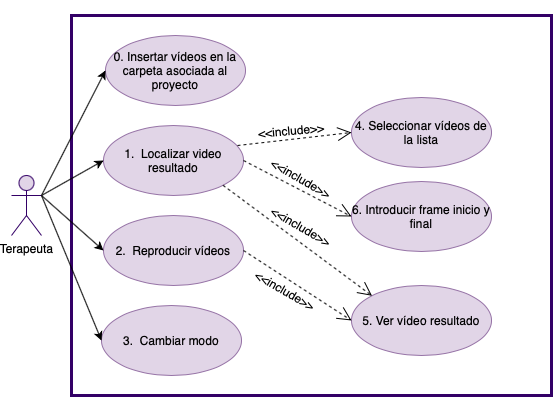
\includegraphics[width=\textwidth]{plantillaLatex-master/img/DiagramaUsoTera copia.png}}
 \caption{Diagrama de casos de uso para el terapeuta.}
 \label{f:casoUsoTerapeuta}
\end{figure}

\begin{figure}[H]
 \centering
  \subfloat{
    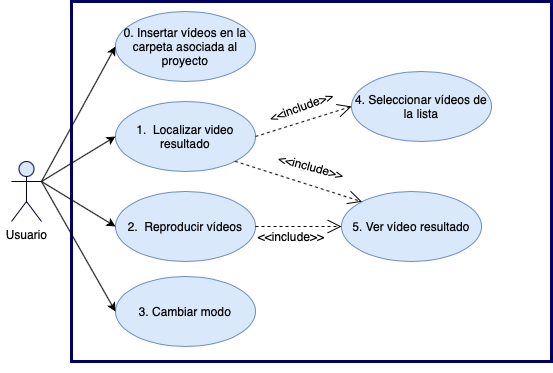
\includegraphics[width=\textwidth]{DiagramaUsoUser.png}}
 \caption{Diagrama de casos de uso para el usuario.}
 \label{f:casoUsoUsuario}
\end{figure}


\tablaSmallSinColores{Caso de uso 0: Insertar vídeos.}{p{3cm} p{.75cm} p{8.5cm}}{tablaUC0}{
  \multicolumn{3}{l}{Caso de uso 0: Insertar vídeos.} \\
 }
 {
  Descripción                            & \multicolumn{2}{p{10.25cm}}{Permite al usuario cargar vídeos de su equipo a la aplicación.} \\\hline
  \multirow{2}{3.5cm}{Requisitos}   &\multicolumn{2}{p{10.25cm}}{RF-4.1} \\\cline{2-3}
                                         & \multicolumn{2}{p{10.25cm}}{RF-4.2} \\\cline{2-3}
                                         & \multicolumn{2}{p{10.25cm}}{RF-4.3} \\\cline{2-3}
                                         & \multicolumn{2}{p{10.25cm}}{RF-4.4}
                                         \\\hline
  Precondiciones                         &  \multicolumn{2}{p{10.25cm}}{Ninguna}   \\\hline
  \multirow{2}{3.5cm}{Secuencia normal}  & Paso & Acción \\\cline{2-3}
                                         & 1    & El usuario o terapeuta introducen los vídeos en el directorio deseado.
  \\\cline{2-3}
                                         & 2    & Al ejecutar la aplicación los vídeos se cargan automáticamente en la barra de selección.
                                         \\\hline
  Postcondiciones                        & \multicolumn{2}{p{10.25cm}}{Vídeos aparecen en cada una de sus listas de selección para posteriormente poder ser mostrados.} \\\hline
  Excepciones                        & \multicolumn{2}{p{10.25cm}}{Ninguna}\\\hline
  Importancia                            & Alta \\\hline
  Urgencia                               & Alta \\
}

\tablaSmallSinColores{Caso de uso 1: Localiza el vídeo.}{p{3cm} p{.75cm} p{8cm}}{tablaUC1}{
  \multicolumn{3}{l}{Caso de uso 1: Localiza el vídeo.} \\
 }
 {
  Descripción                            & \multicolumn{2}{p{10.25cm}}{Permite al usuario localizar el vídeo concreto dentro del vídeo que contiene múltiples ejercicios.} \\\hline
  \multirow{2}{3.5cm}{Requisitos}   &\multicolumn{2}{p{10.25cm}}{RF-1.1} \\\cline{2-3}
                                         & \multicolumn{2}{p{10.25cm}}{RF-1.2} \\\cline{2-3}
                                         & \multicolumn{2}{p{10.25cm}}{RF-1.3} \\\cline{2-3}
                                         & \multicolumn{2}{p{10.25cm}}{RF-1.4} \\\cline{2-3}
                                         \\\hline
  Precondiciones                         &  \multicolumn{2}{p{10.25cm}}{Tener por lo menos algún vídeo concreto y algún vídeo completo cargado}   \\\hline
  \multirow{2}{3.5cm}{Secuencia normal}  & Paso & Acción \\\cline{2-3}
                                         & 1    & El usuario o terapeuta seleccionan el vídeo concreto deseado. \\\cline{2-3}
                                         & 2    & El usuario o terapeuta seleccionan el botón mostrar. \\\cline{2-3}
                                         & 3    & El usuario o terapeuta seleccionan el vídeo concreto deseado. \\\cline{2-3}
                                         & 4    & El usuario o terapeuta seleccionan el botón mostrar. \\\cline{2-3}
                                         & 5    & El usuario o terapeuta seleccionan el botón recortar.\\\cline{2-3}
                                         & 4    & Aparece el vídeo recortado. 
                                         \\\hline
  Postcondiciones                        & \multicolumn{2}{p{10.25cm}}{El vídeo localizado se reproduce automáticamente en la aplicación y se guarda una copia del mismo en la carpeta en la que se ejecuta el proyecto.} \\\hline
  Excepciones                        & \multicolumn{2}{p{10.25cm}}{Ninguna}\\\hline
  Importancia                            & Alta \\\hline
  Urgencia                               & Alta \\
}

\tablaSmallSinColores{Caso de uso 2: Reproducir vídeos.}{p{3cm} p{.75cm} p{8.5cm}}{tablaUC2}{
  \multicolumn{3}{l}{Caso de uso 2: Reproducir vídeos.} \\
 }
 {
  Descripción                            & \multicolumn{2}{p{10.25cm}}{Permite al usuario reproducir y pausar los diferentes vídeos.} \\\hline
  \multirow{2}{3.5cm}{Requisitos}   &\multicolumn{2}{p{10.25cm}}{RF-2.1} \\\cline{2-3}
                                         & \multicolumn{2}{p{10.25cm}}{RF-2.2} \\\cline{2-3}
                                         & \multicolumn{2}{p{10.25cm}}{RF-2.3} \\\cline{2-3}
                                         & \multicolumn{2}{p{10.25cm}}{RF-2.4} \\\cline{2-3}
                                         & \multicolumn{2}{p{10.25cm}}{RF-2.5} \\\cline{2-3}
                                         & \multicolumn{2}{p{10.25cm}}{RF-2.6} \\\cline{2-3}
                                         & \multicolumn{2}{p{10.25cm}}{RF-2.7} \\\cline{2-3}
                                         & \multicolumn{2}{p{10.25cm}}{RF-2.8}
                                         \\\hline
  Precondiciones                         &  \multicolumn{2}{p{10.25cm}}{Tener el vídeo que se desea reproducir o pausar cargado.}   \\\hline
  \multirow{2}{3.5cm}{Secuencia normal}  & Paso & Acción \\\cline{2-3}
                                         & 1    & El usuario o terapeuta seleccionan un vídeo.
  \\\cline{2-3}
                                         & 2    & El usuario o terapeuta pincha sobre el botón play.\\\cline{2-3}
                                         & 3    & Vídeo comienza a reproducirse.\\\cline{2-3}
                                         & 4    & El usuario o terapeuta puede pinchar sobre el botón pause.\\\cline{2-3}
                                         & 5    & El usuario o terapeuta puede pinchar sobre el botón stop.\\\cline{2-3}
                                         & 6    & El vídeo se para.
                                         \\\hline
  Postcondiciones                        & \multicolumn{2}{p{10.25cm}}{Ninguna.} \\\hline
  Excepciones                        & \multicolumn{2}{p{10.25cm}}{Ninguna}\\\hline
  Importancia                            & Alta \\\hline
  Urgencia                               & Alta \\
}

\tablaSmallSinColores{Caso de uso 3: Cambiar modo.}{p{3cm} p{.75cm} p{8.5cm}}{tablaUC3}{
  \multicolumn{3}{l}{Caso de uso 3: Cambiar modo.} \\
 }
 {
  Descripción                            & \multicolumn{2}{p{10.25cm}}{Permite al usuario o al terapeuta cambiar el modo de la aplicación.} \\\hline
  \multirow{2}{3.5cm}{Requisitos}   &\multicolumn{2}{p{10.25cm}}{RF-6.1} \\\cline{2-3}
                                         & \multicolumn{2}{p{10.25cm}}{RF-6.2} \\\cline{2-3}
                                         & \multicolumn{2}{p{10.25cm}}{RF-6.3} \\\cline{2-3}
                                         & \multicolumn{2}{p{10.25cm}}{RF-6.4}
                                         \\\hline
  Precondiciones                         &  \multicolumn{2}{p{10.25cm}}{Ninguna}   \\\hline
  \multirow{2}{3.5cm}{Secuencia normal}  & Paso & Acción \\\cline{2-3}
                                         & 1    & El usuario o terapeuta seleccionan el botón de cambio de modo.
  \\\cline{2-3}
                                         & 2    & Se cambia el modo de la pantalla. 
                                         \\\hline
  Postcondiciones                        & \multicolumn{2}{p{10.25cm}}{Se habilitan o deshabilitan las casillas de los \textit{frames}, se actualizan los vídeos y se cambian los colores.} \\\hline
  Excepciones                        & \multicolumn{2}{p{10.25cm}}{Ninguna}\\\hline
  Importancia                            & Alta \\\hline
  Urgencia                               & Alta \\
}

\tablaSmallSinColores{Caso de uso 4: Seleccionar vídeos de la lista.}{p{3cm} p{.75cm} p{8.5cm}}{tablaUC4}{
  \multicolumn{3}{l}{Caso de uso 4: Seleccionar vídeos de la lista.} \\
 }
 {
  Descripción                            & \multicolumn{2}{p{10.25cm}}{Permite al usuario o terapeuta seleccionar los vídeos concretos o completos que desea reproducir.} \\\hline
  \multirow{2}{3.5cm}{Requisitos}   &\multicolumn{2}{p{10.25cm}}{RF-1.2} \\\cline{2-3}
                                         & \multicolumn{2}{p{10.25cm}}{RF-1.2} \\\cline{2-3}
                                         & \multicolumn{2}{p{10.25cm}}{RF-1.3} \\\cline{2-3}
                                         & \multicolumn{2}{p{10.25cm}}{RF-1.4}
                                         \\\hline
  Precondiciones                         &  \multicolumn{2}{p{10.25cm}}{Que la lista contenga vídeos.}   \\\hline
  \multirow{2}{3.5cm}{Secuencia normal}  & Paso & Acción \\\cline{2-3}
                                         & 1    & El usuario o terapeuta seleccionarán un vídeo concreto de la lista.\\\cline{2-3}
                                         & 2    & El usuario o terapeuta pincha sobre el botón añadir.\\\cline{2-3}
                                         & 3    & El vídeo se carga y se reproduce automáticamente.\\\cline{2-3}
                                         & 4    & El usuario o terapeuta seleccionarán un vídeo completo de la lista.\\\cline{2-3}
                                         & 5    & El usuario o terapeuta pincha sobre el botón añadir.\\\cline{2-3}
                                         & 6    & El vídeo se carga y se reproduce automáticamente.
                                         \\\hline
  Postcondiciones                        & \multicolumn{2}{p{10.25cm}}{Se muestran ambos vídeos cargados y reproduciéndose automáticamente hasta su finalización.} \\\hline
  Excepciones                        & \multicolumn{2}{p{10.25cm}}{Ninguna}\\\hline
  Importancia                            & Alta \\\hline
  Urgencia                               & Alta \\
}

\tablaSmallSinColores{Caso de uso 5: Ver vídeo resultado.}{p{3cm} p{.75cm} p{8.5cm}}{tablaUC5}{
  \multicolumn{3}{l}{Caso de uso 5: Ver vídeo resultado.} \\
 }
 {
  Descripción                            & \multicolumn{2}{p{10.25cm}}{Permite al usuario o terapeuta ver el vídeo final generado.} \\\hline
  \multirow{2}{3.5cm}{Requisitos}   &\multicolumn{2}{p{10.25cm}}{RF-6.3} \\\cline{2-3}
                                         & \multicolumn{2}{p{10.25cm}}{RF-6.4} \\\cline{2-3}
                                         & \multicolumn{2}{p{10.25cm}}{RF-5.1} \\\cline{2-3}
                                         & \multicolumn{2}{p{10.25cm}}{RF-3.1} \\\cline{2-3}
                                         & \multicolumn{2}{p{10.25cm}}{RF-3.2} \\\cline{2-3}
                                         & \multicolumn{2}{p{10.25cm}}{RF-3.5} \\\cline{2-3}
                                         & \multicolumn{2}{p{10.25cm}}{RF-3.6} 
                                         \\\hline
  Precondiciones                         &  \multicolumn{2}{p{10.25cm}}{Haber seleccionado tanto un vídeo concreto como completo. En el caso de no estar en el modo ejemplo será necesario indicar los \textit{frames} por los que se recorta.}   \\\hline
  \multirow{2}{3.5cm}{Secuencia normal}  & Paso & Acción \\\cline{2-3}
                                         & 1    & El usuario o terapeuta seleccionarán un vídeo concreto de la lista.\\\cline{2-3}
                                         & 2    & El usuario o terapeuta seleccionarán un vídeo completo de la lista.\\\cline{2-3}
                                         & 3    & En caso de que sea necesario se especifican los \textit{frames} de inicio y final.\\\cline{2-3}
                                         & 4    & Se pulsa el botón recortar.\\\cline{2-3}
                                         & 5    & El vídeo recortado se guarda automáticamente.
                                         \\\hline
  Postcondiciones                        & \multicolumn{2}{p{10.25cm}}{El vídeo recortado se muestra en la aplicación y se reproduce automáticamente.} \\\hline
  Excepciones                        & \multicolumn{2}{p{10.25cm}}{En caso de que sea necesario especificar el \textit{frame} de inicio y final y no se haya especificado informará del error.}\\\hline
  Importancia                            & Alta \\\hline
  Urgencia                               & Alta \\
}

\tablaSmallSinColores{Caso de uso 6: Introducir \textit{frames} de inicio y final.}{p{3cm} p{.75cm} p{8.5cm}}{tablaUC6}{
  \multicolumn{3}{l}{Caso de uso 6: Introducir \textit{frames} de inicio y final.} \\
 }
 {
  Descripción                            & \multicolumn{2}{p{10.25cm}}{Permite al terapeuta indicar el \textit{frame} de inicio y final del vídeo.} \\\hline
  \multirow{2}{3.5cm}{Requisitos}   &\multicolumn{2}{p{10.25cm}}{RF-3.3} \\\cline{2-3}
                                         & \multicolumn{2}{p{10.25cm}}{RF-3.4} 
                                         \\\hline
  Precondiciones                         &  \multicolumn{2}{p{10.25cm}}{Haber seleccionado tanto un vídeo concreto como completo. }   \\\hline
  \multirow{2}{3.5cm}{Secuencia normal}  & Paso & Acción \\\cline{2-3}
                                         & 1    & El terapeuta seleccionarán un vídeo concreto de la lista.\\\cline{2-3}
                                         & 2    & El terapeuta seleccionarán un vídeo completo de la lista.\\\cline{2-3}
                                         & 3    & El terapeuta especifica los \textit{frames} de inicio y final.\\\cline{2-3}
                                         & 4    & Se pulsa el botón recortar.\\\cline{2-3}
                                         & 5    & El vídeo recortado se guarda automáticamente.
                                         \\\hline
  Postcondiciones                        & \multicolumn{2}{p{10.25cm}}{El vídeo recortado se muestra en la aplicación y se reproduce automáticamente.} \\\hline
  Excepciones                        & \multicolumn{2}{p{10.25cm}}{Ninguna.}\\\hline
  Importancia                            & Alta \\\hline
  Urgencia                               & Alta \\
}


\apendice{Especificación de diseño}

\section{Introducción}

La fase de diseño permite planificar un proyecto para su correcta implementación, desarrollo y evolución. En este apartado se van a exponer los diferentes diseños que se han llevado a cabo para obtener unas buenas soluciones a los problemas planteados. Una de las partes más importantes de este proyecto ha sido la investigación, por lo que el diseño en la mayor parte de este proyecto no ha sido necesaria. 
Los diseños realizados han sido:
\begin{enumerate}
    \item \textbf{Diseño de datos}: en esta parte del diseño se mostrarán todas las estructuras de datos utilizadas y una serie de diagramas para entender la estructura del proyecto. 
    \item \textbf{Diseño procedimental}: en esta parte del diseño se mostrará principalmente la comunicación entre el flujo y las implementaciones realizadas.
    \item \textbf{Diseño arquitectónico}: en esta parte del diseño se especificará la arquitectura del proyecto.
\end{enumerate}

En todos los apartados anteriormente mencionados se expondrá, tanto las fases de diseño de la aplicación, como las fases de diseño del proyecto.

\newpage
\section{Diseño de datos}
\textcolor{blue}{Este apartado cuenta con alguna parte del \textit{Diseño de datos} de José Miguel Ramírez Sanz}

\subsection{Diseño de datos del proyecto}
Este proyecto es mayoritariamente un proyecto de investigación por lo que apenas tiene diseño de datos. En este apartado se va a mostrar un diagrama de clases, como se puede observar en la figura \ref{fig:DiagramaClasesProyecto}, con la implementación final de la clase \texttt{PosicionVF} almacenada en el directorio \texttt{src/process}. El diagrama se ha obtenido del proyecto de José Miguel Ramírez Sanz y se le han añadido las nuevas funcionalidades creadas que son las siguientes:
\begin{enumerate}
    \item \texttt{devuelveAngulos()}: esta función devuelve una matriz con todos los ángulos que componen el esqueleto analizado.
    \item \texttt{devuelvePos()}: esta función devuelve una matriz con todos las posiciones relativas al esqueleto y los ángulos calculados. A estos últimos valores se les añadirá una dimensión extra para subsanar los fallos que genera comparar secuencias con distintas dimensiones. 
    \item \texttt{devuelvePosSuperiores()}: esta función devuelve una matriz que contiene las posiciones de la nariz, hombro izquierdo, hombro derecho, cuello, ángulo del cuello izquierdo, ángulo del cuello derecho, codo izquierdo, codo derecho, mano izquierda, mano derecha, ángulo del codo izquierdo, ángulo del codo derecho, ángulo del hombro izquierdo y ángulo del hombro derecho.
    \item \texttt{devuelvePosInferiores()}: esta función devuelve una matriz que contiene las posiciones de la cadera izquierda, cadera derecha, rodilla izquierda, rodilla derecha, ángulo izquierdo de la cadera, ángulo derecho de la cadera, tobillo izquierdo, tobillo derecho, ángulo izquierdo de la rodilla y ángulo derecho de la rodilla. 
\end{enumerate}

Por otro lado, la clase \texttt{Interfaz} es la que se comunica con el flujo de datos (de ahí su nombre), en ella se carga el modelo para posteriormente crean las posiciones.

Además, en el diagrama se pueden observar las relaciones entre las clases más usadas en el código. En este diagrama se puede observar también como se incorpora la herramienta \textit{Detectron2} en el proyecto (clases \emph{cfg, model\_zoo, Instances y DefaultPredictor)}.


Por otra parte, los ficheros generados para localizar y clasificar la secuencia, localizados en \texttt{src/scripts/deploy} son demasiado sencillos como para generar con ellos un diagrama de clases. Esos ficheros cuentan con las siguientes características:
\begin{enumerate}
    \item \texttt{find\_frames.py}: este fichero hay que ejecutarle pasándole como parámetros dos secuencias. La primera de ellas corresponderá a la secuencia de ejercicios concretos y la segunda a la secuencia compuesta por múltiples ejercicios. Una vez recibe las dos secuencias, extrae las posiciones de los archivos con extensión \textit{.pickle} y ejecuta la búsqueda de secuencias. Finalmente informa al usuario de los \textit{frames} de inicio y final de la secuencia. Adicionalmente se han implementado las funciones que clasifican el ejercicio para informar de que tipo es el ejercicio concreto.
    \item \texttt{classify\_exercises.py}: este fichero hay que ejecutarle pasándole como parámetros la secuencia del ejercicio concreto y devolverá una clasificación en función de si se trata de un ejercicio sobre las partes superiores o inferiores del cuerpo humano.
\end{enumerate}

\begin{figure}[H]
    \centering
    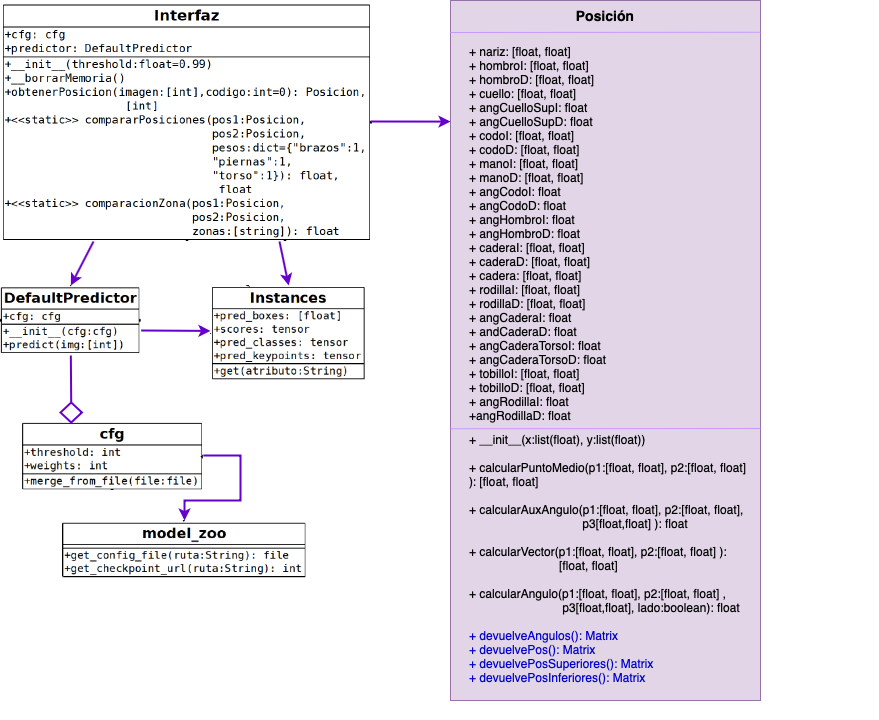
\includegraphics[width=0.9\textwidth]{plantillaLatex-master/img/DiagramaClasesProyecto.png}
    \caption{Diagrama de clases del proyecto.}
    \label{fig:DiagramaClasesProyecto}
\end{figure}

\newpage
\subsection{Diseño de datos de la aplicación}
En este apartado se va a mostrar un diagrama de clases para la aplicación de escritorio, como se puede observar en la figura \ref{fig:DiagramaClasesApp}, en este diagrama se podrán observar las siguientes clases almacenadas en \texttt{app/}:
\begin{enumerate}
    \item \textbf{Window} dentro de \texttt{main.py}, esta clase contiene toda la estructura gráfica de la ventana de la aplicación. En esta clase se pueden apreciar todas las inicializaciones de \textit{frames, labels, botones ...} y las variables que cada uno precisa. Todos estos valores serán almacenados como atributos para poder acceder a ellos con posterioridad desde el resto de clases. 
    \item \textbf{MiddleWindow} dentro de \texttt{MiddleWindow.py}, esta clase tiene como atributo la ventana de inicio. Es la clase encargada de implementar las funciones básicas que debe desarrollar la aplicación, como por ejemplo, mostrar, reproducir o pausar un vídeo, cambiar los colores y habilitar o deshabilitar funcionalidades al cambiar de modo, etc. 
    \item \textbf{PredictWindow} dentro de \texttt{PredictWindow.py}, al igual que la clase anterior, el único atributo que posee es la ventana de inicio. Es la clase encargada de generar el recorte del vídeo, y tiene en cuenta el modo en el que se está trabajando.
\end{enumerate}

\begin{figure}
    \centering
    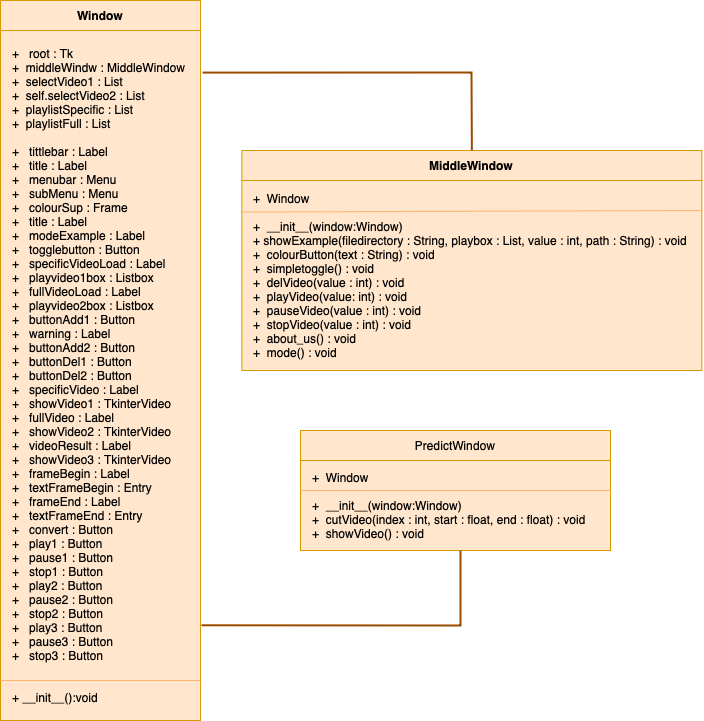
\includegraphics[width=1.1\textwidth]{plantillaLatex-master/img/DiagramaClasesApp.png}
    \caption{Diagrama de clases de la aplicación.}
    \label{fig:DiagramaClasesApp}
\end{figure}

\newpage
\section{Diseño procedimental}
\textcolor{blue}{Este apartado es una ampliación del Diseño de datos de José Luis Garrido Labrador}

\subsection{Diseño procedimental del proyecto}
En este apartado se van a mostrar un par de diagramas de secuencias. En la figura \ref{fig:DiagramaSeqProyecto}, se muestra el proceso general de la aplicación. Este programa contiene una clase \texttt{Ingestor} que se encarga de encolar los \textit{frames} recibidos, y procesarlos. En este proyecto los \textit{frames} vienen procedentes de un único vídeo y lo que programa realiza es ejecutar ese vídeo en bucle por lo que el proceso únicamente acabaría cuando el usuario finaliza el programa. 
\begin{figure}[H]
    \centering
    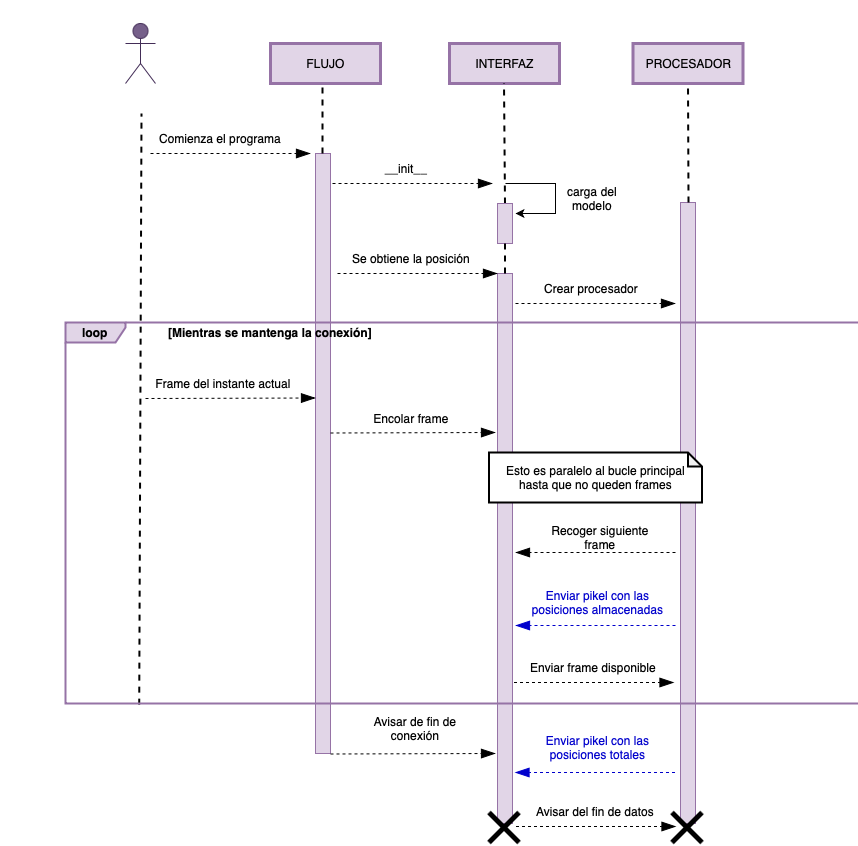
\includegraphics[width=0.9\textwidth]{plantillaLatex-master/img/DiagramaSeqProyecto.png}
    \caption{Diagrama de secuencias de la parte encargada de obtener las posiciones.}
    \label{fig:DiagramaSeqProyecto}
\end{figure}

Por otra parte, en la figura \ref{fig:DiagramaSeqProy2} se puede observar el proceso que se genera para obtener los \textit{frames} de inicio y final y la clasificación del ejercicio. 

\begin{figure}[H]
    \centering
    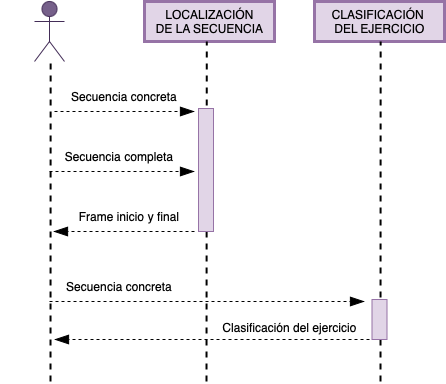
\includegraphics[width=0.7\textwidth]{plantillaLatex-master/img/DiagramaSeqProy2.png}
    \caption{Diagrama de secuencias de la parte encarga de de localizar las secuencias.}
    \label{fig:DiagramaSeqProy2}
\end{figure}


\subsection{Diseño procedimental de la aplicación}
En el diagrama de secuencias que se puede apreciar en la figura \ref{fig:DiagramaSeqApp}, se muestran las tareas principales de la aplicación de escritorio: cargar, reproducir, pausar y detener un vídeo, cambiar el modo de la aplicación y generar un recorte del vídeo que contiene la secuencia de ejercicios completa.

Como se puede apreciar la única diferencia entre el \textit{modo ejemplo ON} y el \textit{modo ejemplo OFF} es que en el segundo hay que especificar los \textit{frames} por los que se desea recortar el vídeo, mientras que en el caso anterior lo hace automáticamente.

\begin{figure}[H]
    \centering
    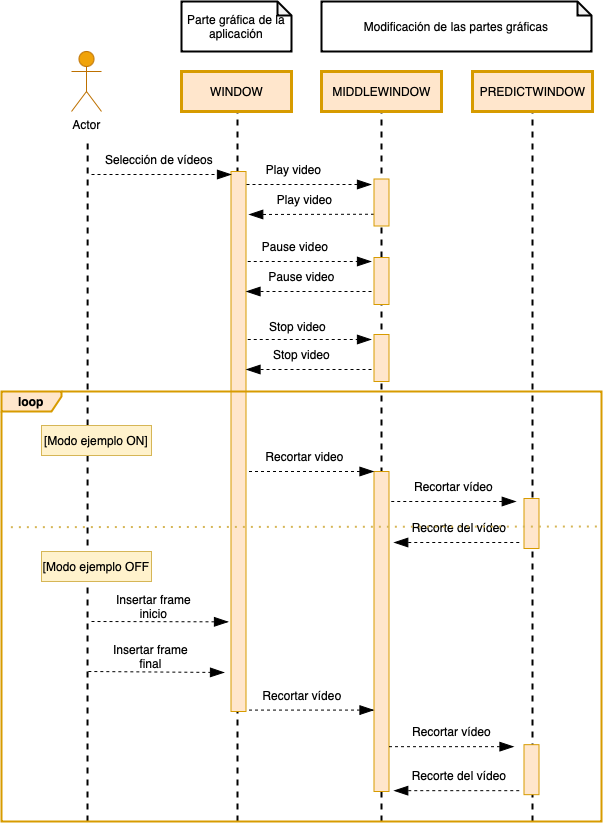
\includegraphics[width=\textwidth]{plantillaLatex-master/img/DiagramaSeqApp.png}
    \caption{Diagrama de secuencias de la aplicación.}
    \label{fig:DiagramaSeqApp}
\end{figure}


\newpage
\section{Diseño arquitectónico}
\textcolor{blue}{Este apartado ha sido extraído del \textit{Diseño de datos arquitectónicos} de José Luis Garrido Labrador}

\subsection{Diseño arquitectónico del proyecto}
Una parte muy esencial de este proyecto es el uso de y despliegue de máquinas virtuales \textit{Docker}. Concretamente hay cuatro tipos de imágenes \textit{Docker}. La primera se
encarga de la serialización de los \textit{frames} y lanzan el \textit{script} de \textit{Python} de
encolado, esta máquina se crea y destruye a voluntad de las conexiones de los pacientes. La segunda y tercera imágenes son el servicio de \textit{Zookeeper} y de \textit{Kafka}. Estas imágenes no se duplican en caso de cambios en las conexiones, únicamente se crean o borran colas. Por último, la cuarta imagen es la transformación del flujo. Se crean o se destruyen según las conexiones de los pacientes y se parametrizan para que consuman un flujo concreto y hagan un procesamiento concreto. El diagrama de despliegue de las máquinas virtuales \textit{docker} se puede observar en la \ref{fig:imgDock}.

\begin{figure}[H]
    \centering
    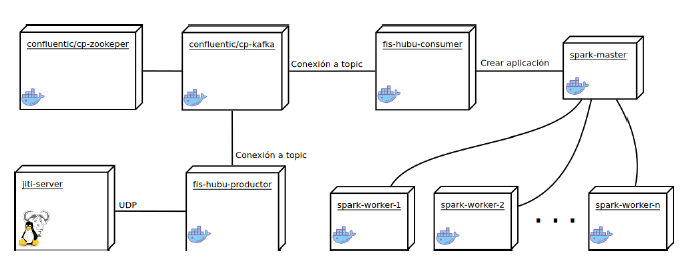
\includegraphics[width=\textwidth]{plantillaLatex-master/img/ImgDocker.png}
    \caption{Diagrama de despliegue de las máquinas virtuales \textit{docker}.}
    \label{fig:imgDock}
\end{figure}

Por otra parte, se ha creado un diagrama con la estructura de los directorios más relevantes del proyecto y se puede observar en la figura \ref{fig:EstructuraDirectoriosSrc}. En esta estructura destacan los directorios:
\begin{enumerate}
    \item \texttt{src/scripts/deploy}: contiene todos los ficheros necesarios para desplegar los servidores e imágenes \textit{Docker}. Además cuenta con los ficheros específicos de este proyecto que localizan y clasifican las secuencias.
    \item \texttt{src/process}: contiene todos los ficheros necesarios para la obtención de las secuencias.
    \item \texttt{src/pruebas}: contiene los distintos \textit{notebooks} generados para explicar las fases del proyecto, a si como muchas de las secuencias generadas y vídeos realizados.
\end{enumerate}

\begin{figure}[H]
    \centering
    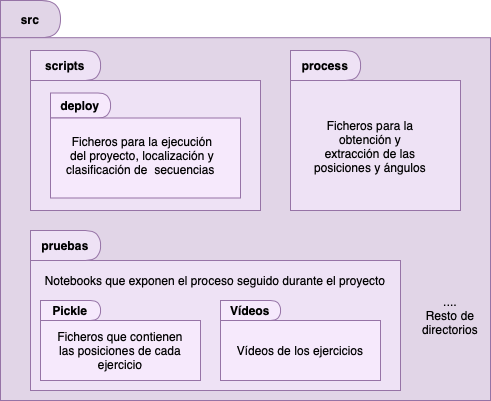
\includegraphics[width=0.55\textwidth]{plantillaLatex-master/img/EstructuraDirectoriosSrc.png}
    \caption{Diagrama de paquetes de la aplicación.}
    \label{fig:EstructuraDirectoriosSrc}
\end{figure}

\subsection{Diseño arquitectónico de la aplicación}
En este apartado se definirá la estructura en paquetes de la aplicación. Como se puede observar en la figura \ref{fig:EstructuraDirectorisApp} la distribución es muy simple. Se almacenan los vídeos en diferentes directorios dentro de la carpeta en la que se encuentran las clases de dicha aplicación. Según el directorio en el que se encuentren cada uno de los vídeos, se cargarán en una sección u otra de la aplicación.

\begin{figure}[H]
    \centering
    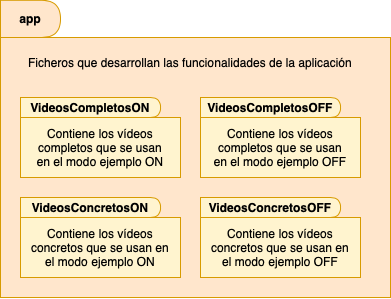
\includegraphics[width=0.55\textwidth]{plantillaLatex-master/img/EstructuraDirectorisApp.png}
    \caption{Diagrama de paquetes de la aplicación.}
    \label{fig:EstructuraDirectorisApp}
\end{figure}

\apendice{Documentación técnica de programación}

\section{Introducción}
En este apartado se mostrarán los distintos requisitos e instrucciones necesarias para la instalación y comprensión del proyecto. Para ello se deberá tener en cuenta:
\begin{enumerate}
    \item \textbf{Estructura de directorios}: se mostrará la estructura general del proyecto. Este apartado también se puede observar en el repositorio de  \textit{GitHub} que contendrá, a parte de la estructura de directorios, las tareas realizadas. 
    \item \textbf{Manual del programador}: manual en el que se exponen los pasos a seguir para poder continuar con el proyecto. 
    \item \textbf{Compilación, instalación y ejecución del proyecto}: manual que abarca las instrucciones básicas para poder ejecutar el proyecto.  
    \item \textbf{Pruebas del sistema}, explicación de las distintas pruebas realizadas y de como lanzarlas.
\end{enumerate}

\section{Estructura de directorios}
En este subapartado se comentará la estructura del contenido del proyecto. Es la misma que la que se puede apreciar en el repositorio de \texttt{\textit{GitHub}}\footnote{https://github.com/lnc1002/TFG-Evaluacion-Ejercicios-Rehabilitacion.git}:

\dirtree{%
.1 /.
.2 app.
.3 VideosCompletos\_Ej\_OFF.
.3 VideosCompletos\_Ej\_ON.
.3 VideosConcretos\_Ej\_OFF.
.3 VideosConcretos\_Ej\_ON.
.2 doc.
.3 Vídeos.
.3 Látex.
.4 img.
.4 tex.
.2 src.
.3 dockers.
.4 fishubu.
.5 base.
.5 enviroment.
.4 kafka.
.4 spark.
.5 base.
.5 master.
.5 worker.
.3 process.
.4 model.
.4 testvideos.
.3 prueba.
.3 pruebas.
.4 Pickle.
.4 vídeos.
.4 img.
.3 scripts.
.4 deploy.
.4 helpers.
.3 tools.
.4 jupyter.
.4 videos.
.5 processed.
.5 raw.
.2 README.md.
.2 LICENSE.
.2 gitignore.
}

Como se puede observar, de la raíz cuelgan las carpetas \texttt{app, src, doc} y tres documentos con las siguientes funcionalidades:
\begin{enumerate}
    \item \texttt{README.md}: documento que se encuentra en la raíz del repositorio de \textit{GitHub} y aparecerá en más directorios. Este fichero muestra información relativa al proyecto y a los ficheros que contiene el directorio en el que se ubica. Está compuesto por un resumen y unas instrucciones básicas de como está estructurado el contenido del proyecto.
    \item \texttt{LICENSE}: documento que contiene la licencia del proyecto en \textit{GitHub}.
    \item \texttt{.gitignore}: documento que especifica que archivos o directorios no se desean subir al repositorio. 
\end{enumerate}

\subsection{Documentación}
Una vez comentada la estructura de ficheros se va a exponer la estructura de los directorios que cuelgan desde la raíz del proyecto. La carpeta \texttt{doc} contiene toda la documentación del proyecto y tiene la siguiente estructura:
\dirtree{%
.1 doc.
.2 Latex.
.3 img.
.3 tex.
.2 Videos.
.2 Readme.md.
}

Dentro del directorio \texttt{Latex} se encuentra toda la documentación de memoria y anexos realizada sobre \LaTeX. En la carpeta \texttt{/doc/Latex/img} se localizan todas las imágenes y diagramas usados en este proyecto. Tanto una gran cantidad de imágenes como de diagramas han sido realizados con la herramienta \textit{Diagrams.net} \cite{wiki:drawio}. 

En el directorio \texttt{Videos} se encuentran unos breves vídeos del funcionamiento de como ejecutar el proyecto, obtener los \textit{frames} resultantes a partir de los \textit{pickle} generados y como interactuar con la aplicación de escritorio. 

\newpage
\subsection{Código}
La carpeta \texttt{src} contiene todos los ficheros y directorios necesarios tanto para ejecutar el programa como para la localización de las secuencias. En concreto vamos a exponer el contenido del directorio \texttt{/src/scripts/deploy/}:
\dirtree{%
.1 src.
.2 scripts.
.3 deploy.
.4 new-stream.
.4 start-server.
.4 stop-server.
.4 stop-stream.
.4 classify\_exercises.py.
.4 find\_frames.py.
}

Los dos últimos ficheros son los que se han implementado para poder localizar la secuencia o clasificar el ejercicio una vez haya terminado el proceso de extracción de posiciones.

Por otra parte, el directorio \texttt{/src/pruebas/} contiene:
\dirtree{%
.1 src.
.2 pruebas.
.3 C1\_Pruebas\_paquetes\_DTW.ipynb.
.3 C2\_Buscar\_Subsecuencia.ipynb.
.3 C3\_Busqueda\_y\_agrupacion\_de\_secuencia\_SIMILAR.ipynb.
.3 C4\_Busqueda\_multiples\_secuencias.ipynb.
.3 C5\_Busqueda\_inicio\_y\_final.ipynb.
.3 C6\_Pruebas\_busqueda\_angulos.ipynb.
.3 C7\_Pruebas\_busqueda\_posiciones.ipynb.
.3 C8\_Pruebas\_recortando\_frames.ipynb.
.3 C9\_Pruebas\_clasificacion\_movimientos.ipynb.
.3 C10\_Resultados\_finales.ipynb.
.3 Pickle.
.4 Posiciones\_inferiores.
.4 Posiciones\_superiores.
.4 Posiciones\_completas.
.4 Angulos\_completos.
.3 vídeos.
.3 img.
.3 README.md.
}

Como se puede observar dentro de este directorio se encuentran los diferentes \textit{notebooks} que se han empleado para mostrar las pruebas realizadas durante todo el proceso del proyecto. Además en el directorio \texttt{/src/pruebas/Pickle} se encuentran almacenadas gran parte de las secuencias generadas y en el directorio \texttt{/src/pruebas/vídeos} algunos de los vídeos creados para dichas pruebas. 


\subsection{Aplicación}
La carpeta \textbf{app} contiene todos los ficheros y directorios necesarios para poder ejecutar la aplicación de escritorio y su estructura es la siguiente:
\dirtree{%
.1 app.
.2 VideosCompletos\_Ej\_OFF.
.2 VideosCompletos\_Ej\_ON.
.2 VideosConcretos\_Ej\_OFF.
.2 VideosConcretos\_Ej\_ON.
.2 .gitignore.
.2 MiddleWindow.py.
.2 PredictWindow.py.
.2 main.py.
.2 README.md.
.2 requirements.txt.
}

\section{Manual del programador}

Todo el proyecto ha corrido sobre la máquina \textit{gamma} del equipo \textit{ADMIRABLE} de la Universidad de Burgos y para poder llevar a cabo las ejecuciones se han tenido que instalar una serie de programas sobre el entorno de \textit{Ubuntu}.
Muchos de estos programas han sido instalados mediante el comando \textit{wget} y el entorno final ha quedado con los siguientes programas y versiones:
\begin{enumerate}
    \item \textbf{Anaconda}: es una distribución de \textit{Python} utilizada para el desarrollo científico tanto gráfico como analítico \cite{wiki:anaconda}. En este proyecto se ha utilizado la versión \textbf{conda 4.11.0}.
    \item \textbf{NVIDIA}: es un \textit{software} que ofrece una amplia gama de posibilidades para la construcción o aceleración de aplicaciones \cite{wiki:nvidia}. En este proyecto se ha utilizado la versión \textbf{460.80}.
    \item \textbf{CUDA}: es una plataforma de computación paralela  y un modelo de programación desarrollados por \textit{NVIDIA} \cite{wiki:cuda}. En este proyecto se ha utilizado la versión de CUDA \textbf{ 11.2}.
    \item \textbf{Detectron2}: es una plataforma para la detección de objetos ~\cite{wu2019detectron2}.En este proyecto se ha utilizado la versión 0.6. Para más información sobre \textit{Detectron2} visitar el apartado de la memoria \textit{Técnicas y herramientas}.
    \item \textbf{Tensorflow}: es una plataforma de código abierto que cuenta con una amplia cantidad de herramientas y recursos para el aprendizaje automático \cite{wiki:tensorflow}. En este proyecto se ha utilizado la versión \textbf{2.8.0}.
\end{enumerate}


\subsection{\textit{Script} de despliegue}
\textcolor{blue}{Este apartado ha sido extraído del \textit{Script} de despliegue de José Luis Garrido Labrador}

Para el despliegue de los servicios mediante \textit{Docker} se han creado cuatro \textit{scripts} localizados en la carpeta \texttt{src/scripts/deploy}. Estos códigos en \textit{Bash} son los siguientes:
\begin{enumerate}
    \item \textbf{start-server}: se encarga de instanciar los diferentes servicios.
    \begin{lstlisting}[language=Bash]
 Sintaxis
	    start-server <Carpeta de salida> <N. de CPU master> <N. de workers> <N. de CPU por worker> <Memoria por worker>
    \end{lstlisting}
    \item \textbf{stop-server}: detiene todos los servicios.
    \begin{lstlisting}[language=Bash]
 Sintaxis
	    stop-server
    \end{lstlisting}
    \item \textbf{new-stream}: \label{cap:newstream} genera un nuevo flujo completo que se va a procesar. El funcionamiento es transparente. Recibe los parámetros para el \texttt{emitter.py} y para el \texttt{consumer.py}. Por seguridad es preferible solamente modificar los parámetros de gestión del flujo y no los de comunicación. Devuelve el identificador del flujo. Es importante este valor para poder cerrarlo después.
    \begin{lstlisting}[language=Bash]
 Sintaxis
    	new-stream "Parámetros emitter.py" "Parámetros consumer.py"
    	# Es muy importante mantener las comillas
    \end{lstlisting}
    \item \textbf{stop-stream}: detiene todos los procesos sobre un flujo concreto.
    \begin{lstlisting}[language=Bash]
 Sintaxis
	    stop-stream <ID del flujo>
    \end{lstlisting}
\end{enumerate}


\subsection{\textit{Script} de análisis}
Para la comparación de secuencias se han creado dos \textit{scripts}:
\begin{enumerate}
    \item \textbf{find\_frames.py}: localiza el patrón de referencia dentro de la secuencia de mayor tamaño y devolverá los \textit{frames} en los que se ha iniciado y finalizado la supuesta secuencia encontrada. Por último devolverá también una clasificación del tipo de ejercicio realizado.
    \begin{lstlisting}[language=Bash]
 Sintaxis
	    find_frames.py <secuencia del ejercicio concreto> <secuencia con varios ejercicios>
    \end{lstlisting}
    \item \textbf{classify\_exercises.py}: informará del tipo de ejercicio que se está realizando en el vídeo pasado como argumento.
    \begin{lstlisting}[language=Bash]
 Sintaxis
	    classify_exercises.py <secuencia del ejercicio concreto> 
    \end{lstlisting}
\end{enumerate}

\newpage
\section{Compilación, instalación y ejecución del proyecto}
\textcolor{blue}{Parte de este apartado ha sido extraído del apartado de \textit{Compilación, instalación y ejecución del proyecto} de José Luis Garrido Labrador}

Como se ha mencionado anteriormente, en la carpeta \texttt{src/scripts/deploy} se encuentran los \textit{scripts} para instalar el proyecto y poder ejecutarlo.

Para que los \textit{scripts} se ejecuten correctamente es necesario que se corran sobre un sistema operativo GNU/Linux con el servicio \textit{Docker} y la extensión \textit{Nvidia container toolkit} ~\cite{toolkitnvidiadocker} instalados. Adicionalmente se necesitará que la máquina donde se vayan a ejecutar los \textit{workers} disponga de una tarjeta gráfica \textit{Nvidia} instalada con soporte para \textit{CUDA} 10.2. 

Es posible que sea necesario cambiar el fichero \textit{Dockerfile} de la \texttt{carpeta dockers/fishubu/base} para que use los drivers de la tarjeta gráfica del equipo sobre el que se lanza la imagen \textit{docker}.


Antes de lanzar los servicios es importante haber creado previamente las imágenes maestras \textbf{(orden build)} para los diferentes \textit{dockers}. Desde la carpeta deploy:
\begin{lstlisting}[language=Bash]
docker build -f ../../dockers/fishubu/base/Dockerfile -t fishubu-base:1.0.0 ../../
docker build -f ../../dockers/fishubu/enviroment/Dockerfile -t fishubu-env:1.0.0 ../../
docker build ../../dockers/spark/base -t spark-base-fis:2.4.5
docker build ../../dockers/spark/master -t spark-master-fis:2.4.5
docker build ../../dockers/spark/worker -t spark-worker-fis:2.4.5
\end{lstlisting}

El orden de ejecución de los \textit{scripts} es el siguiente:

\begin{enumerate}
	\item \textbf{Ejecutar \texttt{start-server}} para que los servicios de \textit{Kafka} y \textit{Spark} estén activos y den soporte a los flujos que lo necesiten.
	\item \textbf{Ejecutar \texttt{new-stream}} recibiendo como parámetros la configuración deseada para el emisor y para el consumidor.  Este devuelve el identificador del flujo, será necesario para pedir el cierre del flujo.
\end{enumerate}

Para detener el flujo los pasos son los siguientes:
\begin{enumerate}
	\item \textbf{Ejecutar \texttt{stop-stream}} para cada flujo arrancado.
	\item \textbf{Ejecutar \texttt{stop-server}} y se detendrán todos los servicios.
\end{enumerate}

Para localizar la secuencia y clasificar los ejercicios el orden en el que se realicen las ejecuciones es indiferente. Por otra parte, tampoco es necesario que se esté corriendo el programa que extrae las secuencias, simplemente se necesitará tener algunas de ellas almacenadas:
\begin{enumerate}
    \item \textbf{Ejecutar \texttt{find\_frames.py}} para la extracción de la secuencia.
    \item \textbf{Ejecutar \texttt{classify\_exercises.py}} para la clasificación del ejercicio.
\end{enumerate}

\section{Fallos y soluciones} \label{cap:FallosSoluciones}
En este apartado se van a exponer algunos de los errores por los que se ha visto comprometido el proyecto, sus causas y sus posibles soluciones. 

Los fallos que producidos durante el trascurso de las ejecuciones son almacenados en diferentes ficheros. Por una parte se encuentran los ficheros de \textit{\textbf{log}} ubicados en el directorio \texttt{/tmp/fishubulogs}. Para consultar estos ficheros será necesario indicar el identificador correspondiente al flujo lanzado, de esta forma los comandos a ejecutar serían los siguientes:
\begin{enumerate}
    \item Consultar el fichero \textit{\textbf{log-error}}:
    \begin{lstlisting}[language=Bash]
 Sintaxis
	    cd /tmp/fishubulogs/log-error-{id-stream} 
    \end{lstlisting}
    \item Consultar el fichero \textit{\textbf{log}}:
    \begin{lstlisting}[language=Bash]
 Sintaxis
	    cd /tmp/fishubulogs/log-{id-stream} 
    \end{lstlisting}
\end{enumerate}

Otros errores serán almacenados en la carpeta \textit{\textbf{logs}} de cada máquina \textit{docker} ejecutada. Para poder observar estos errores será necesario adentrarse en el contender del que se quiera obtener información, esta acción se realiza mediante alguno de los siguientes comandos:
\begin{lstlisting}[language=Bash]
 Sintaxis
	    docker exec -it <container_name> bash}
\end{lstlisting}
\begin{lstlisting}[language=Bash]
 Sintaxis
	    docker exec -it <container_id> bash}
\end{lstlisting}

\subsection{Fallos de memoria}
\subsubsection{Fallos en la caída del flujo}
\textcolor{blue}{Parte del fallo redactado por Jose Luis Garrido Labrador y ampliado por Lucía Núñez Calvo}

Si la caída del flujo deja una excepción del tipo \textit{\textbf{Caused by: java.io.EOFException}}, como se puede observar en la figura \ref{f:EOFException}, o se observa el siguiente mensaje de error dentro del \textit{script} {/tmp/fishubulogs/log-error-{id-stream}} \textit{\textbf{StreamingContext: StreamingContext has already been stopped}} como se puede apreciar en la figura \ref{f:StreamingContext}, implica que los datos que debe procesar el flujo son mayores que los que caben en memoria.
Para solucionar este problema será necesario dar más memoria a cada \textit{worker}. El valor recomendado es de 2 GiB por cada núcleo de \textit{worker} pero se puede aumentar si el usuario lo considera oportuno.

\begin{figure}[H]
 \centering
\subfloat{
    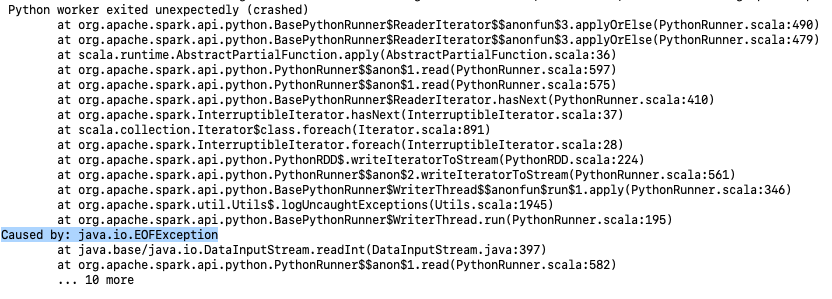
\includegraphics[width=\textwidth]{plantillaLatex-master/img/EOFException.png}}
 \caption{Error de tipo \textit{Caused by: java.io.EOFException}.}
 \label{f:EOFException}
\end{figure}

\begin{figure}[H]
 \centering
\subfloat{
    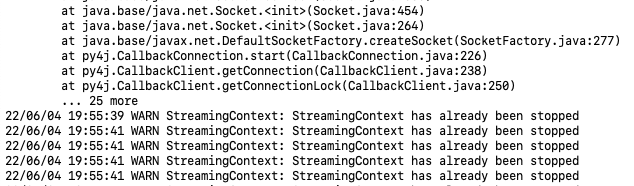
\includegraphics[width=\textwidth]{plantillaLatex-master/img/StreamingContext.png}}
 \caption{Error de tipo \textit{StreamingContext: StreamingContext has already been stop-ped}.}
 \label{f:StreamingContext}
\end{figure}


\subsubsection{Fallos con \textit{Docker}}

En caso de que se proceda al lanzamiento de los contenedores y la salida por pantalla sea \textit{\textbf{The server is not running}}, como se observa en la figura \ref{f:servernotrunning}, el problema puede ser que se haya agotado la memoria en el directorio \texttt{/var/cache/apt/archives/}. Para solventar este problema se tendrá que ejecutar siguiente el comando:
\begin{lstlisting}[language=Bash]
 Sintaxis
	    docker system prune --all
\end{lstlisting}

Tras su ejecución se deberán restaurar las imágenes (orden build).

\begin{figure}[H]
 \centering
\subfloat{
    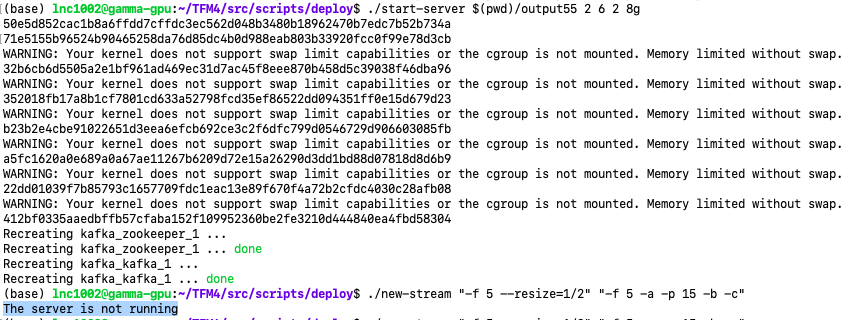
\includegraphics[width=\textwidth]{plantillaLatex-master/img/ServerNot.png}}
 \caption{Error de tipo \textit{The server is not running}.}
 \label{f:servernotrunning}
\end{figure}

\subsection{Error de permisos}
Si el proyecto se está ejecutando sobre la máquina \textit{gamma} del grupo \textit{ADMIRABLE} de la Universidad de Burgos y tras intentar lanzar el servidor aparecen numerosos mensajes de tipo \textit{\textbf{Get permission denied while trying to connect to the Docker daemon socket at unix}}, como el que se puede apreciar en la imagen \ref{f:permissionDe}, quiere decir que el usuario no está presente en el grupo \textit{docker}.

\begin{figure}[H]
 \centering
\subfloat{
    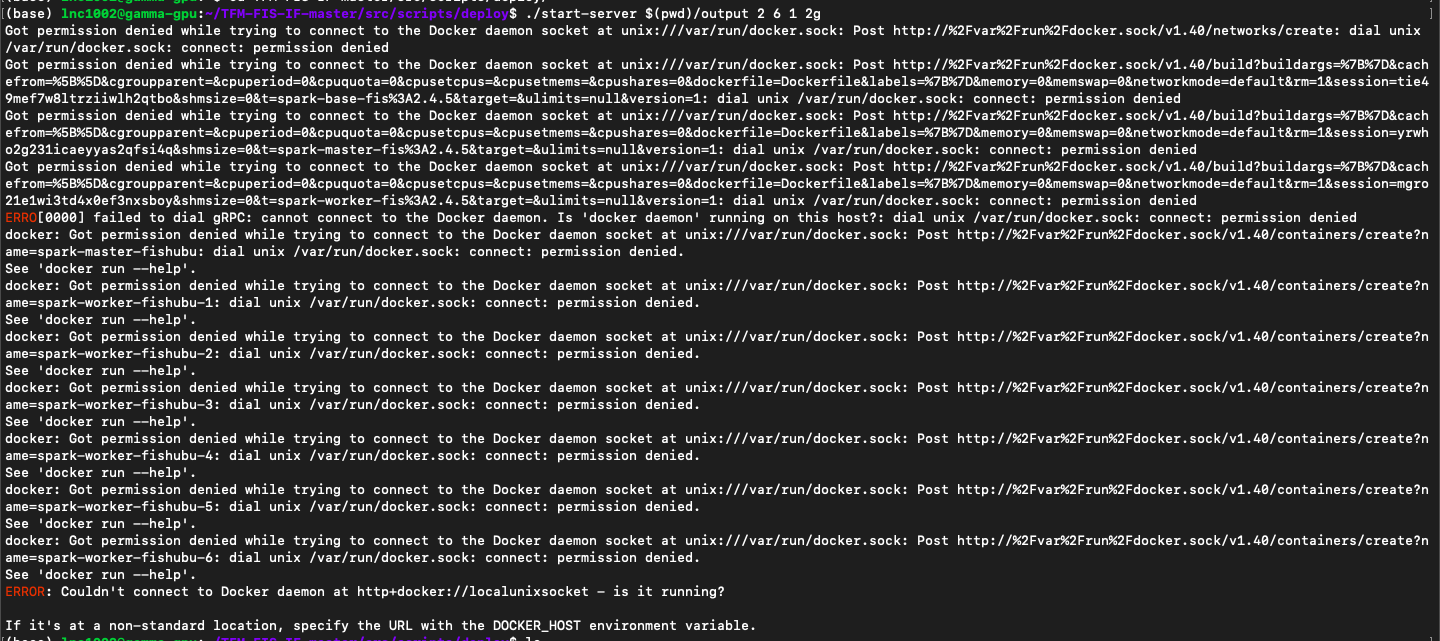
\includegraphics[width=\textwidth]{plantillaLatex-master/img/permissionDenied.png}}
 \caption{Error de tipo \textit{Get permission denied while trying to connect to the Docker daemon socket at unix}.}
 \label{f:permissionDe}
\end{figure}

Para solventar este problema, un administrador del sistema deberá ejecutar el siguiente comando:
\begin{lstlisting}[language=Bash]
 Sintaxis
	    usermod -a -G docker nombre-usuario
\end{lstlisting}

\subsection{Los fotogramas no se procesan}
\textcolor{blue}{Parte del fallo redactado por Jose Luis Garrido Labrador y ampliado por Lucía Núñez Calvo}

Si los fotogramas no se procesan y observa la existencia del fichero de \texttt{log/notprocesslog} en los \textit{workers}, significa que ha existido un error mientras se procesaba el fotograma. En el mismo \textit{\textbf{log}} se encuentra el origen del fallo y probablemente se deberá a que el fichero de \texttt{extraOpt.py} incluye información errónea o una ruta incorrecta.

Para solucionar esto se debe volver a cargar el fichero \texttt{extraOpt.py} y por tanto se han de volver a construir  las imágenes \emph{(orden build)} desde la \texttt{fishubu-env}. En el caso de que el error persista, usar el flag \emph{--no-cache} a
la hora de reconstruir las imágenes.

\subsection{Error de \textit{Kafka}}

Algunos de los errores que pueden aparecer ante un usuario impaciente son los siguiente, como se puede apreciar en la imagen \ref{f:kafkaerror}: 
\begin{enumerate}
    \item \textit{Error while executing topic command : Replication factor: 1 larger than available brokers: 0.
ERROR org.apache.kafka.common.errors.
InvalidReplicationFactorException: Replication factor: 1 larger than available brokers: 0. (kafka.admin.TopicCommand)}
    \item \textit{WARN [AdminClient clientId=adminclient-1] Connection to node -1 (localhost/127.0.0.1:9092) could not be established. Broker may not be available. (org.apache.kafka.clients.NetworkClient)}
\end{enumerate}

\begin{figure}[H]
 \centering
\subfloat{
    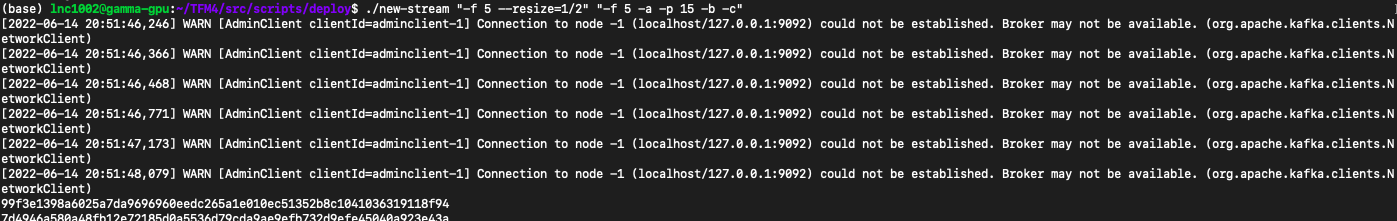
\includegraphics[width=\textwidth]{plantillaLatex-master/img/errorKafka.png}}
 \caption{Error de tipo \textit{kafka}.}
 \label{f:kafkaerror}
\end{figure}

Estos errores únicamente le informan al usuario de que no ha dejado suficiente tiempo para que se cargue \textit{Kafka} correctamente. El tiempo de carga puede variar por múltiples factores, por esa razón puede, que tras lanzar el servidor se intente crear un flujo y no nos muestre el error, mientras que en otras ocasiones si lo haga. Por ello, es recomendable dejar trascurrir unos segundos desde que se lanza el servidor. 

En caso de que aparezca este error, únicamente se pararía el flujo creado y se volverían a lanzar los contenedores. 


\subsection{Errores de versión de \textit{Nvidia}}
\textcolor{blue}{Redactado por Jose Luis Garrido Labrador}

Si a la hora de ejecutar el flujo, en el arranque ocurre una excepción del tipo \textit{\textbf{forward compatibility was attempted}} indica que la versión instalada de \textit{Nvidia} sobre \textit{docker} no es compatible con la versión instalada
en el equipo.

Para solucionarlo es necesario cambiar el fichero \emph{Dockerfile} de la carpeta \texttt{src/dockers/fishubu/base} y cambiar la versión que se instala por la que se tiene en el equipo. Es necesario que al menos sea la versión 440.

\subsection{Error con la conexión a \textit{Nvidia}}
\textcolor{blue}{Redactado por Jose Luis Garrido Labrador}

Si el flujo al iniciar da el error \textit{\textbf{could not select device driver}} significa que la extensión de \textit{docker} para la compatibilidad con \textit{Nvidia} no está instalada o no se ha reiniciado el servicio de \textit{docker} desde que se instaló.

Se soluciona instalando la extensión de \textit{docker «docker-nvidia»} y reiniciando el servicio.


\section{Pruebas del sistema}
Como se ha podido observar, el proyecto se ha dividido en dos fases principales. Una primera fase fue el análisis de librerías y la segunda fase fue condensar todo lo investigado en la implementación del objetivo del proyecto.

Prácticamente todas las pruebas se han corrido sobre distintos \textit{notebooks} ya que esta herramienta permite organizar de una manera muy intuitiva cómoda y visual los resultados obtenidos, pero ¿qué se entiende por pruebas?. 

Un aspecto a tener en cuenta es la dificultad de ejecutar pruebas unitarias en minería de datos. Para ejecutar una prueba se debe saber de manera previa el resultado, en nuestro caso este resultado sólo se consigue mediante un análisis visual por parte del usuario. Es el propio programador el que tiene que comprobar si la secuencia obtenidas se corresponde con la secuencia esperada. Este resultado se ha podido comprobar de dos maneras:
\begin{enumerate}
    \item \textbf{Pruebas mediante código}: el procedimiento a seguir para realizar este tipo de pruebas es muy sencillo. Tras analizar el vídeo que contiene la secuencia de ejercicios completos, localizamos visualmente el vídeo que queremos encontrar y nos quedamos con el instante de tiempo en el que comienza y finaliza. El siguiente paso es una mera regla de tres. Si se tienen un total de $X$ \textit{frames} y el vídeo cuenta con una duración de $Z$ instantes de tiempo, el momento justo en el que empieza o finaliza el ejercicio concreto encontrado dentro del vídeo que contiene todos los ejercicios será igual a
    \begin{equation}
        \frac{frame\_encontrado*Z}{X}
    \end{equation}
    \item \textbf{Pruebas mediante la aplicación de escritorio}: el procedimiento a realizar en este caso es más sencillo porque el cálculo anterior ya se encuentra implementado en la aplicación. En este caso será necesario cargar tanto el vídeo concreto como el vídeo que comprende toda la secuencia de ejercicios y proceder a recortar el vídeo. Visualizando el recorte en la aplicación se podrá comprobar lo bien o mal que se está detectando la secuencia.
\end{enumerate}

Finalmente comentar que las pruebas han sido esenciales en este proyecto para poder seleccionar el mejor algoritmo para el objetivo perseguido, es decir, el algoritmo que consiga localizar una amplia colección de secuencias en un tiempo relativamente aceptable. 


 

\apendice{Documentación de usuario}

\section{Introducción}
En este apartado se detallarán las principales funcionalidades que ofrece la aplicación de escritorio a si como todo lo necesario para que los usuarios puedan instalar y ejecutar la aplicación fácilmente. 

\section{Requisitos de usuarios}
Para poder correr la aplicación será necesario tener instalado \textit{Python}, al menos la versión 3.8.8 e instalar los requerimientos especificados en el fichero \texttt{app/requirements.txt}. Esta aplicación está pensada para ser ejecutada sobre el sistema operativo \textit{Windows}.

\section{Instalación}
Los pasos básicos para instalar el proyecto y con ende la aplicación son los siguientes:
\begin{enumerate}
    \item Clonar repositorio e ir al directorio \texttt{app/}.
    \item Comprobar que se encuentran almacenados algunos vídeos en las diferentes carpetas que contiene el directorio \texttt{app/}.
    \item Ejecutar el comando:
    \newpage
    \begin{lstlisting}[language=Bash]
 Sintaxis
        install.cmd 
    \end{lstlisting}
    o en su defecto
    \begin{lstlisting}[language=Bash]
 Sintaxis
        pip install -r requirements.txt
    \end{lstlisting}
\end{enumerate}

Finalmente para ejecutar la aplicación:
Para ejecutar la aplicación:
\begin{lstlisting}[language=Bash]
 Sintaxis
    python main.py
\end{lstlisting}


\section{Manual del usuario}

\subsection{Cambiar el modo de la aplicación}
Para cambiar el modo de la aplicación observar figuras \ref{fig:app1} \ref{fig:app2}. Al cambiar de modo se ejecutarán las siguientes acciones:
\begin{enumerate}
    \item \textbf{Cambio de colores}: si el usuario se encuentra en \textit{modo ejemplo ON} aparecerá una ventana con tonos verdes azulados y azules, mientras que si el usuario se encuentra en \textit{modo ejemplo OFF} los tonos serán de color lila. Al cambiar el color de toda la aplicación dependiendo del modo de ejecución en el que se encuentre el usuario se logra evitar confusiones sobre en que modo se encuentra. 
    \item \textbf{Cambio del texto del botón}: es imprescindible que el usuario sepa en todo momento en que modo de ejecución se encuentra por lo que el cambio de colores no es suficiente, mediante el botón \textit{ON/OFF} se informará del modo en el que se encuentra la aplicación. 
    \item \textbf{Bloqueo o desbloqueo de casillas}: las casillas por las que se inserta el \textit{frame} de inicio y final aparecerán bloqueadas si el usuario se encuentra en \textit{modo ejemplo ON} ya que no necesitará hacer uso de ellas.
    \item \textbf{Actualización de vídeos}: si la aplicación cambia de modo, se actualizarán los vídeos mostrados en las listas de selección. Cada modo puede contener diferentes vídeos.
    \item \textbf{Descarte de vídeos}: si la aplicación está reproduciendo un vídeo y se ejecuta un cambio de modo, automáticamente descartará el vídeo.
\end{enumerate}

\begin{figure}[H]
    \centering
    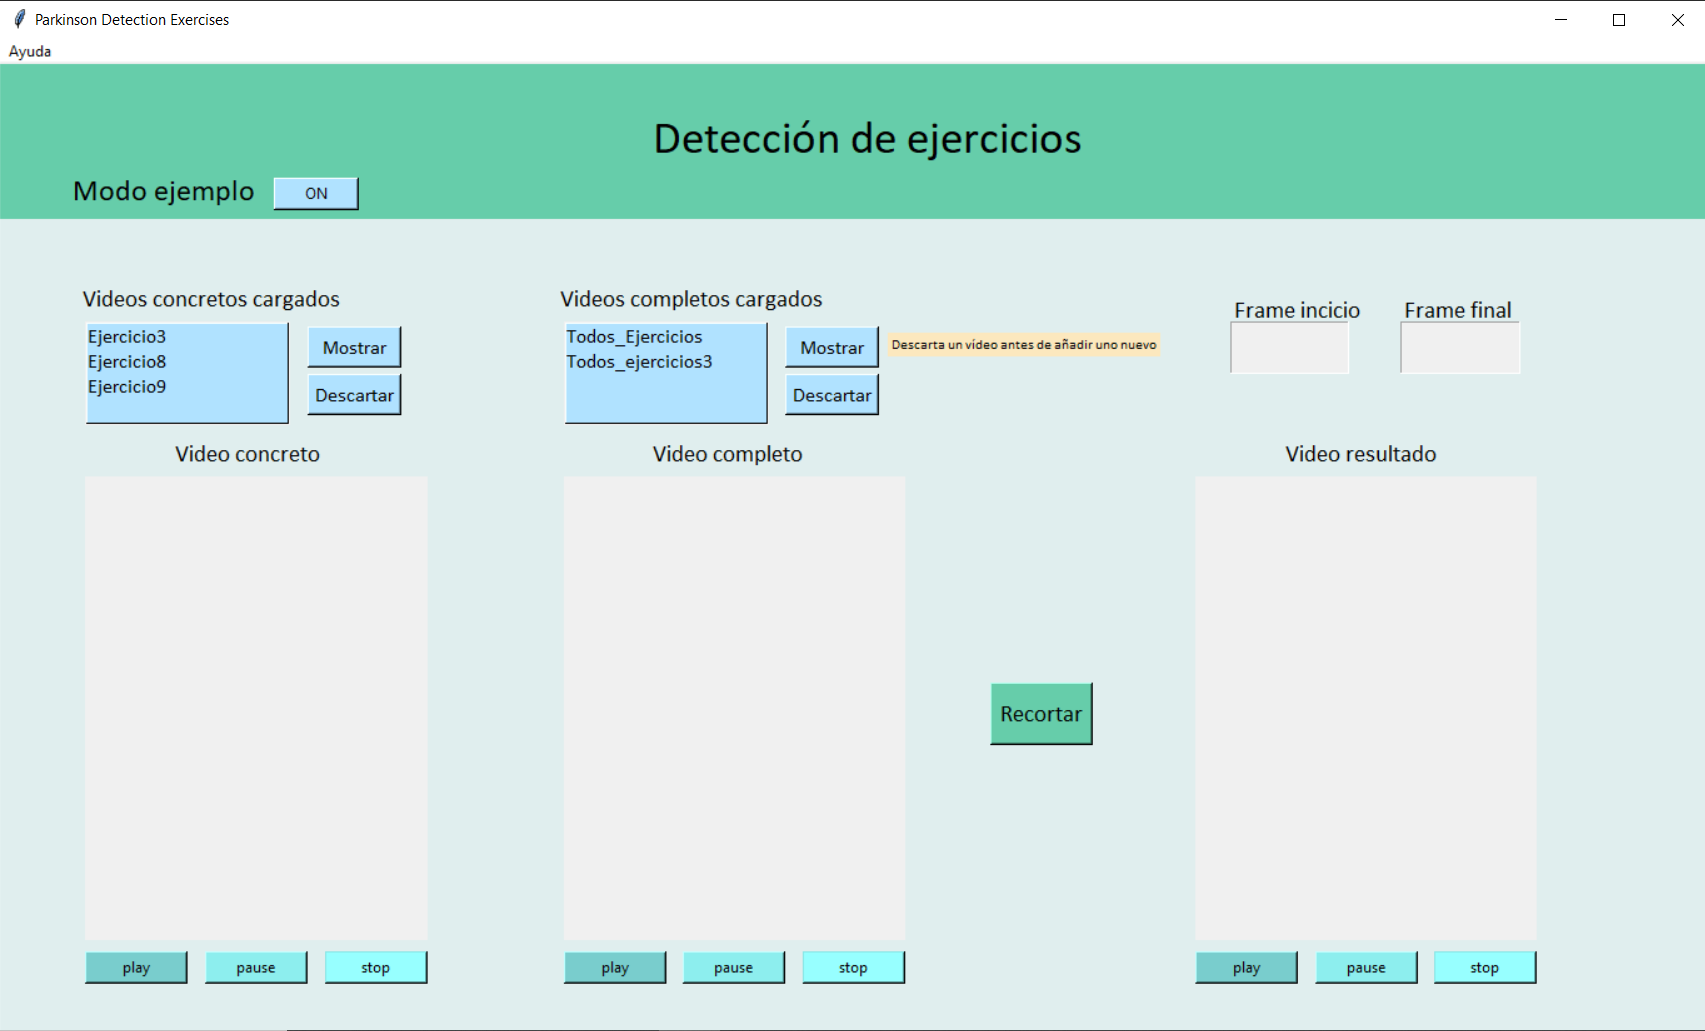
\includegraphics[width=0.8\textwidth]{plantillaLatex-master/img/app1.PNG}
    \caption{Aplicación en modo ejemplo ON.}
    \label{fig:app1}
\end{figure}

\begin{figure}[H]
    \centering
    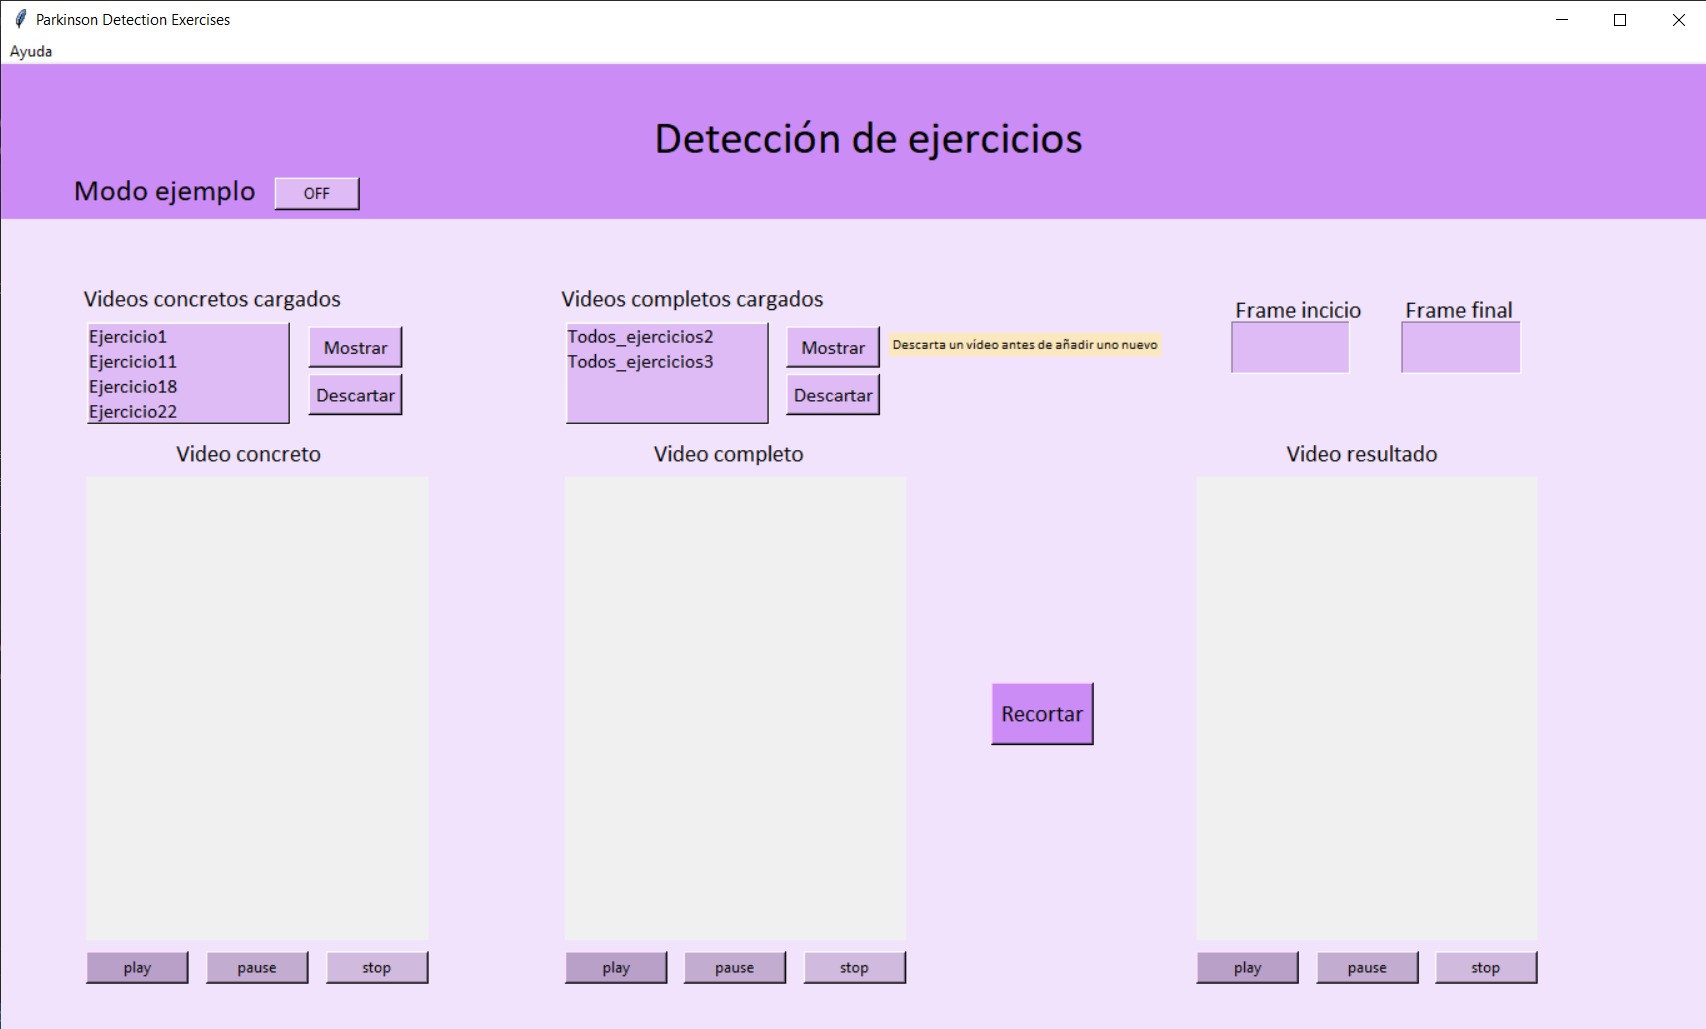
\includegraphics[width=0.8\textwidth]{plantillaLatex-master/img/app2.PNG}
    \caption{Aplicación en modo ejemplo OFF.}
    \label{fig:app2}
\end{figure}

\subsection{Mostrar y borrar un vídeo}
Una vez se arranca la aplicación de escritorio, los vídeos son cargados automáticamente por la aplicación y mostrados en la barra de selección. 

\subsubsection{Mostrar un vídeo}
Para mostrar un vídeo ver figura \ref{fig:app3}. Al mostrar un vídeo se ejecutarán las siguientes acciones:
\begin{enumerate}
    \item \textbf{Seleccionar un vídeo}: lo primero que se deberá hacer es escoger un vídeo de los mostrados en la lista de selección.
    \item \textit{Pinchar en el botón \textbf{Mostrar}}: tras seleccionar un vídeo y seguidamente pinchar en este botón, la aplicación cargará el vídeo seleccionado en su ventana correspondiente y empezará con su reproducción. 
    \item \textbf{Descartar vídeos previos}: si se desea cargar un vídeo cuando ya hay otro en ejecución, es muy importante descartar el vídeo previo. En caso de no realizarse correctamente esta acción, el vídeo seleccionado no se cargará.
\end{enumerate}

\begin{figure}[H]
    \centering
    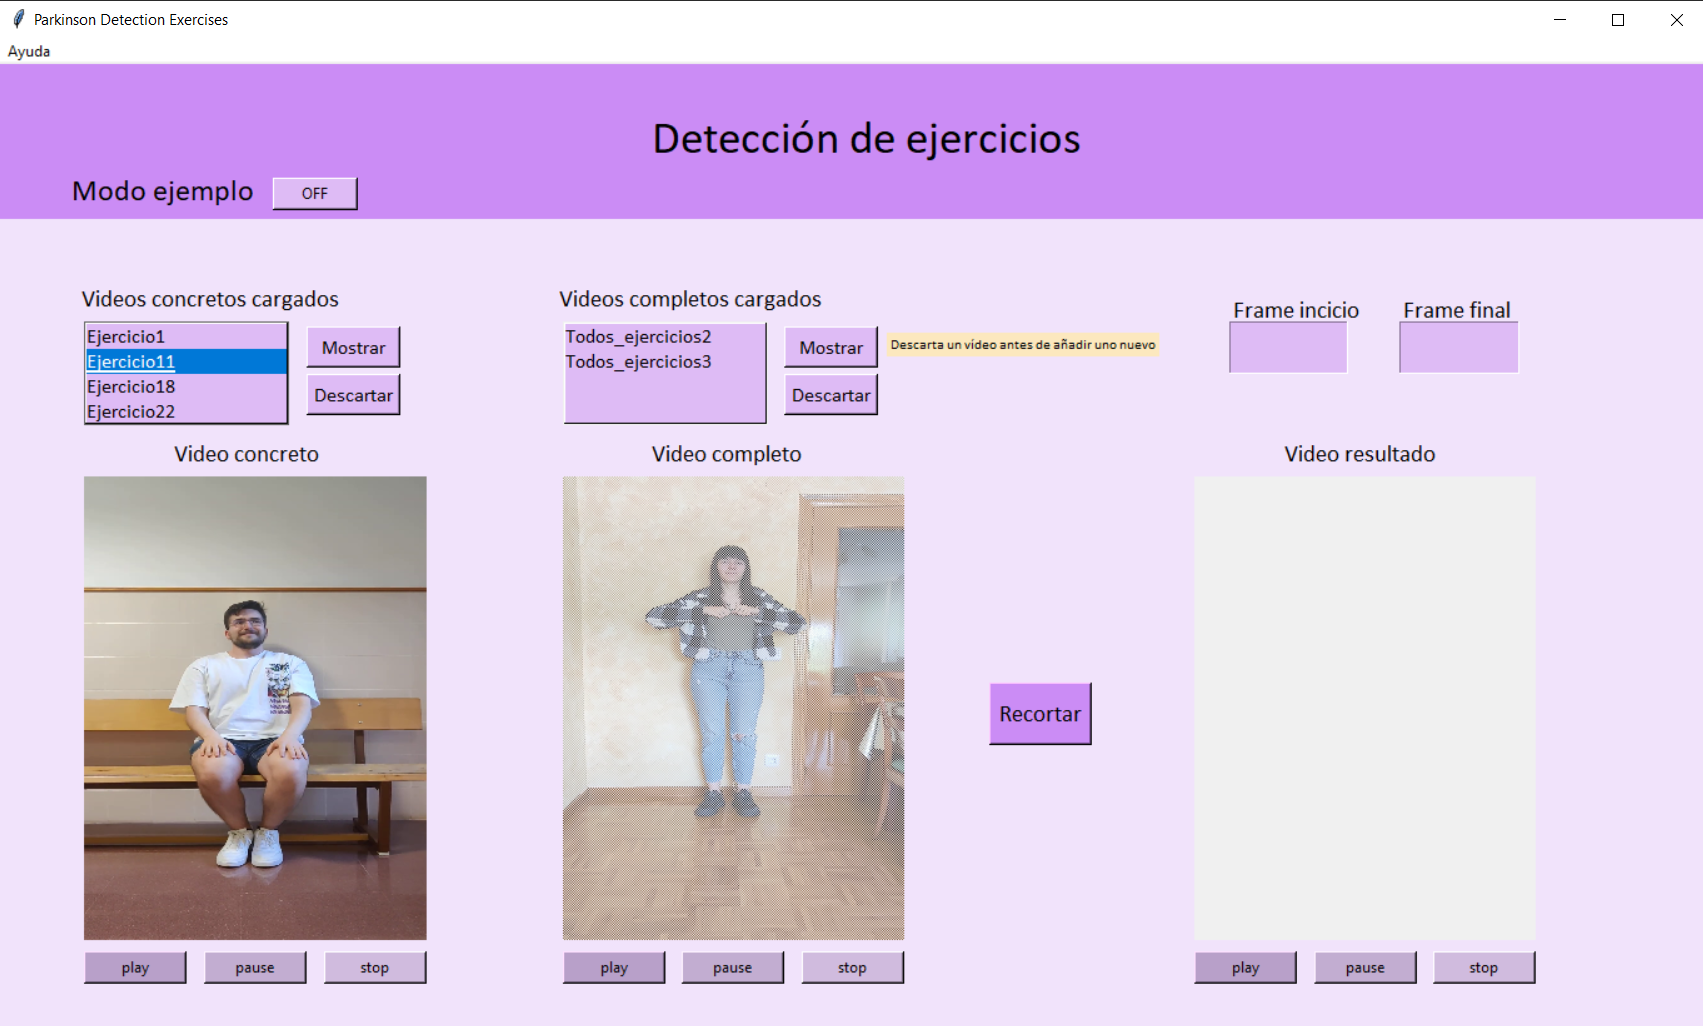
\includegraphics[width=\textwidth]{plantillaLatex-master/img/app3.PNG}
    \caption{Carga y descarte de vídeos.}
    \label{fig:app3}
\end{figure}

\subsubsection{Descartar un vídeo}
Para descartar un vídeo ver figura \ref{fig:app3}. Al descartar un vídeo se ejecutarán las siguientes acciones:
\begin{enumerate}
    \item \textbf{Seleccionar el vídeo}: para que el vídeo se descarte correctamente se deberá seleccionar el vídeo que está en ejecución y que se desea eliminar. 
    \item \textbf{Pinchar en el botón \textit{Descartar}}: una vez seleccionado el vídeo se pulsará este botón. Esta acción simplemente deja de reproducirlo en su ventana correspondiente, pero no elimina el vídeo de la lista de selección,
    por esta razón se pueden cargar y descartar tantas veces como se desee.
    \item \textbf{EL vídeo se bloqueará}: como se ha comentado anteriormente los vídeos no son eliminados por completo si no que únicamente se bloquean y dejan de reproducirse. Una vez el vídeo está bloqueado se podrán añadir nuevos vídeos.
\end{enumerate}

\subsection{Interaccionar con el vídeo}
Una vez esté cargado un vídeo, se podrá pausar y reanudar tantas veces como el usuario desee. 

\subsubsection{Reproducir un vídeo}
Para reproducir un vídeo se tendrán en cuenta estas sencillas acciones:
\begin{enumerate}
    \item \textbf{Pinchar en el botón \textit{play}}: los vídeos pausados o detenidos únicamente empezarán  a reproducirse pulsando este botón. 
    \item \textbf{EL vídeo empezará a reproducirse}: si el vídeo se encuentra pausado o detenido, ya sea porque el usuario ha presionado el botón \textit{stop} o porque la duración del vídeo ha llegado a su fin, una vez se pincha sobre el botón \textit{play}, empezará su reproducción.
\end{enumerate}

\newpage
\subsubsection{Pausar un vídeo}
Para pausar un vídeo se tendrán en cuenta estas sencillas acciones:
\begin{enumerate}
    \item \textbf{Pinchar en el botón \textit{pause}}: este botón únicamente permitirá la pausa del vídeo en reproducción. No ejecutará el vídeo de nuevo al hacer doble \textit{click}.
    \item \textbf{EL vídeo se pausará}: el vídeo permanecerá pausado hasta que se ejecute una acción de reproducción. 
\end{enumerate}

\subsubsection{Detener un vídeo}
Para detener un vídeo se tendrán en cuenta estas sencillas acciones:
\begin{enumerate}
    \item \textbf{Pinchar en el botón \textit{stop}}: este botón únicamente permitirá la detención inmediata del vídeo en reproducción. No ejecutará el vídeo de nuevo al hacer doble \textit{click}. 
    \item \textbf{EL vídeo se parará}: el vídeo permanecerá detenido hasta que se ejecute una acción de reproducción. En este caso, el vídeo comenzará desde el instante inicial.
\end{enumerate}


\subsection{Recortar un vídeo}
Los vídeos se podrán recortar en ambos modos de ejecución. En las imágenes \ref{fig:app5} y \ref{fig:app4} se puede observar como el ejercicio realizado por el vídeo que simula al terapeuta es localizado en el vídeo que simula al paciente y posteriormente muestra dicho resultado. 

\subsubsection{Recortar un vídeo en modo ejemplo ON}
Para recortar un vídeo en \textit{modo ejemplo ON} ver figura \ref{fig:app5} y tener en cuenta las siguientes acciones:
\begin{enumerate}
    \item \textbf{Seleccionar un vídeo concreto}: se deberá escoger el vídeo que se desea encontrar dentro de la secuencia de ejercicios.
    \item \textbf{Seleccionar un vídeo completo}: también se deberá escoger el vídeo del que se desea obtener el recorte.
    \item \textbf{Pinchar en el botón \textit{Recortar}}: para ver el resultado final del recorte se deberá pulsar en este botón. En cuanto el vídeo recortado sea cargado empezará a reproducirse.
\end{enumerate}
\begin{figure}[H]
    \centering
    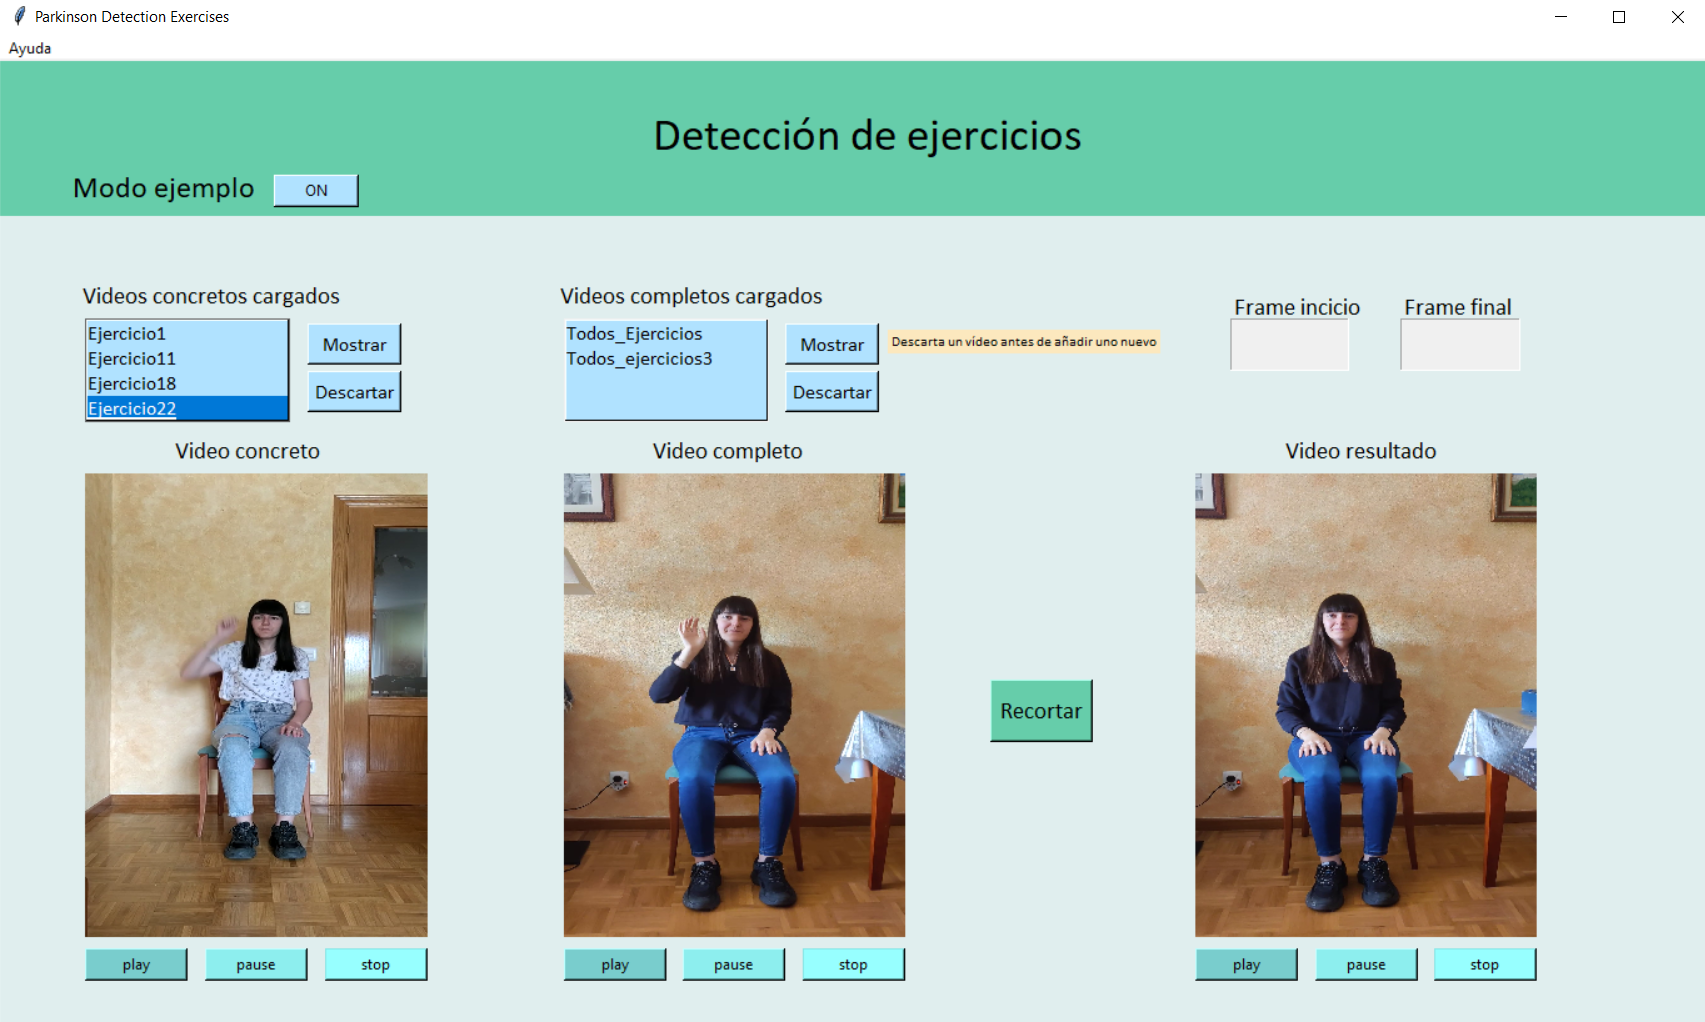
\includegraphics[width=\textwidth]{plantillaLatex-master/img/app5.PNG}
    \caption{Recorte de vídeos en modo ejemplo ON.}
    \label{fig:app5}
\end{figure}

\subsubsection{Recortar un vídeo en modo ejemplo OFF}
Para recortar un vídeo en \textit{modo ejemplo OFF} ver figura \ref{fig:app4} y tener en cuenta las siguientes acciones:
\begin{enumerate}
    \item \textbf{Seleccionar un vídeo concreto}.
    \item \textbf{Seleccionar un vídeo completo}.
    \item \textbf{Indicar el \textit{frame} de inicio}: para el generar el recorte será necesario indicar el punto de inicio en la casilla correspondiente.
    \item \textbf{Indicar el \textit{frame} de final}: también será necesario especificar el punto en el que se desea que finalice el resultado. 
    \item \textbf{Pinchar en el botón \textit{Recortar}}: una vez se tienen ambos valores cargados, tras seleccionar este botón aparecerá el vídeo resultado reproduciéndose automáticamente.
\end{enumerate}
\begin{figure}
    \centering
    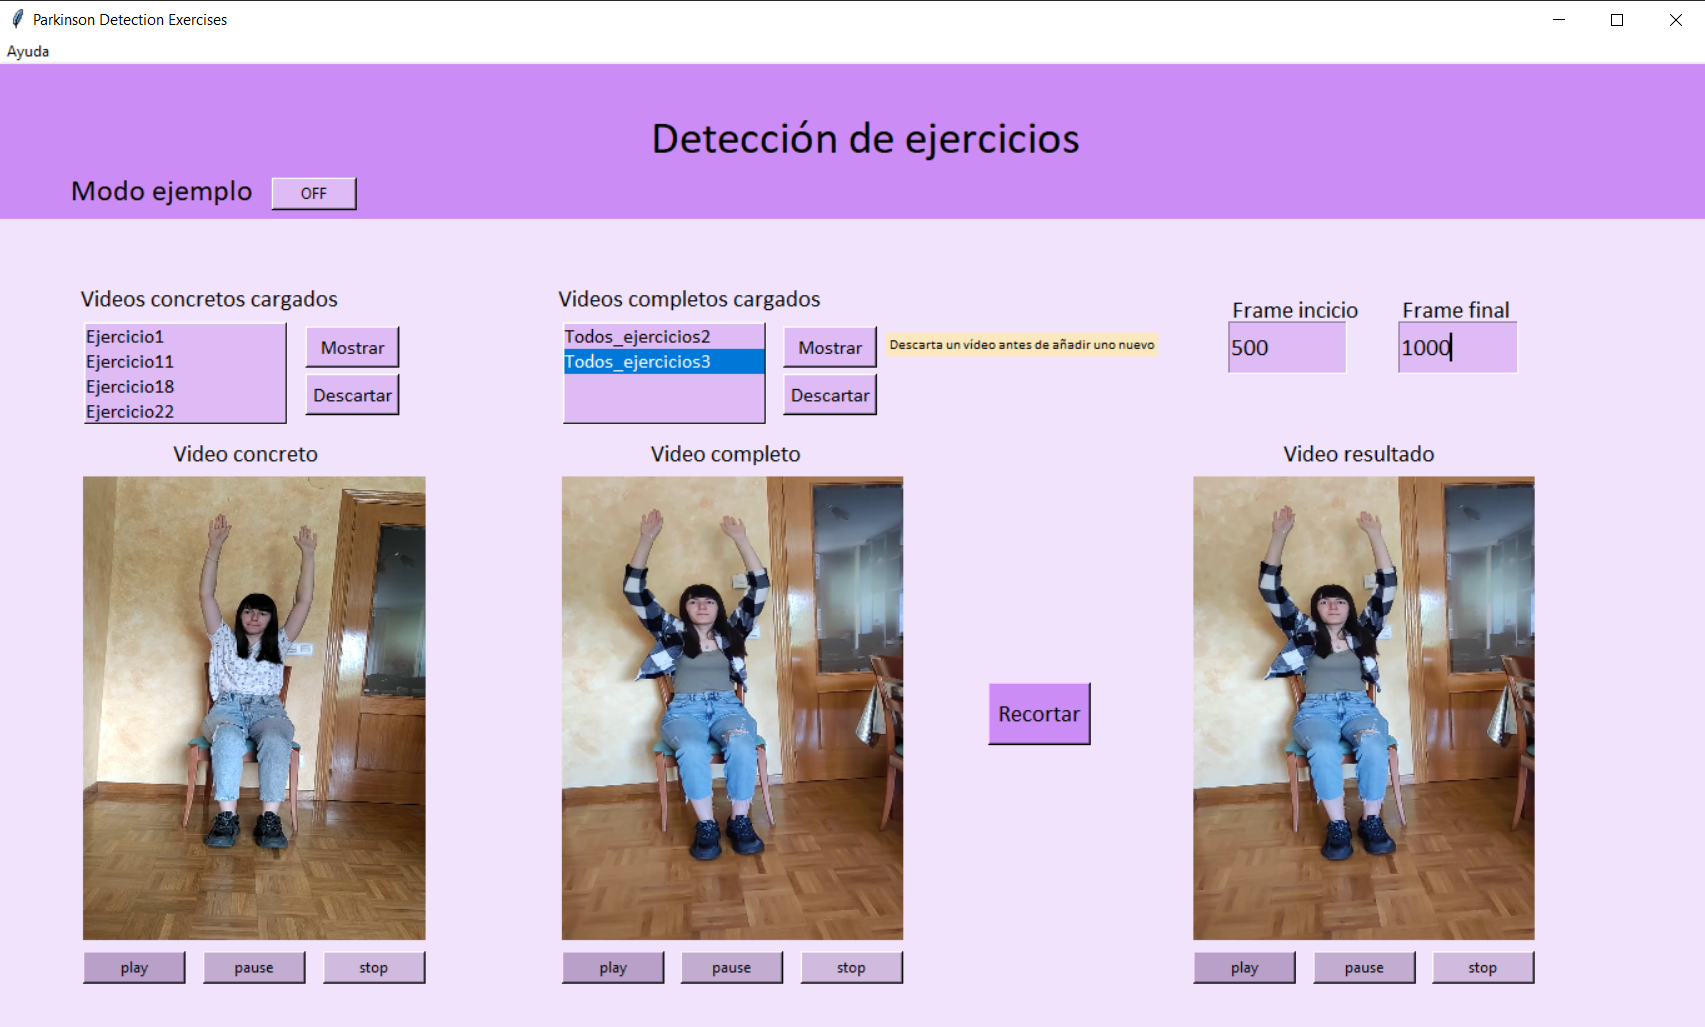
\includegraphics[width=0.9\textwidth]{plantillaLatex-master/img/app4.PNG}
    \caption{Recorte de vídeos en modo ejemplo OFF.}
    \label{fig:app4}
\end{figure}

\subsection{Excepciones e información de la aplicación}
Finalmente comentar los siguientes aspectos relevantes e la aplicación:
\begin{enumerate}
    \item Si el usuario se encuentra en el \textit{modo ejemplo ON} y selecciona el botón recortar sin haber especificado los \textit{frames} de inicio y de final, mostrará el siguiente aviso:
    \begin{figure}[H]
        \centering
        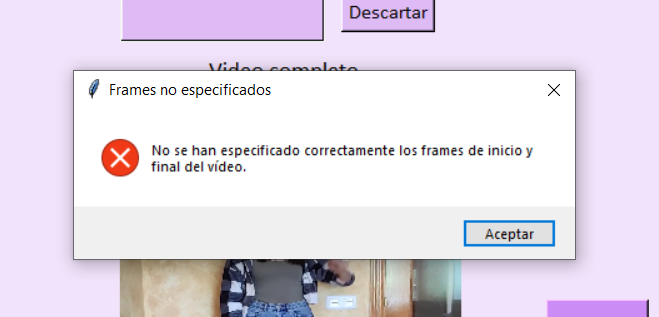
\includegraphics[width=0.35\textwidth]{plantillaLatex-master/img/NoFrames.PNG}
        \caption{Aviso de falta de frames.}
    \label{fig:app4}
\end{figure}
    \item Si se selecciona el desplegable \textbf{\textit{Ayuda}} se mostrarán las opciones \textit{Proyecto} y \textit{Modo ejemplo} que mostrarán la siguiente información:
\begin{figure}[H]
 \centering
  \subfloat {
   \label{f:gatos}
    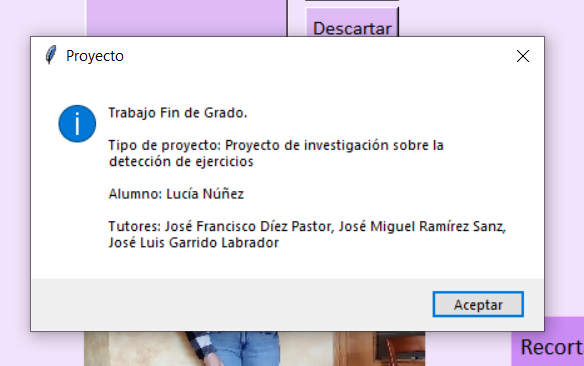
\includegraphics[width=0.295\textwidth]{plantillaLatex-master/img/ProyectInf.PNG}}
  \subfloat {
   \label{f:perros}
    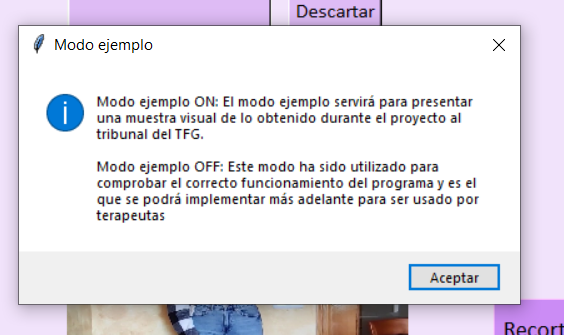
\includegraphics[width=0.32\textwidth]{plantillaLatex-master/img/ExampleMode.PNG}}
 \caption{Detección de animales usando diferentes algoritmos.}
 \label{f:animales1}
\end{figure}

    
\end{enumerate}



\bibliographystyle{plain}
\bibliography{bibliografiaAnexos}

\end{document}
